\documentclass[man,12pt,floatsintext,donotrepeattitle]{apa7}

\usepackage[american]{babel}
\usepackage{csquotes}
\usepackage{amsmath,amssymb}
\usepackage{amsthm}
\usepackage{booktabs}
\usepackage{graphicx}
\usepackage{xcolor}
\usepackage{subcaption}
\usepackage[most]{tcolorbox}
\usetikzlibrary{positioning, arrows.meta, fit, decorations.pathreplacing}
\usepackage{needspace}
\usepackage[style=apa,backend=biber]{biblatex}
\addbibresource{refs.bib}
\usepackage{nameref}
\hypersetup{
  hidelinks,
  pdftitle={A New Family of Operators on Cellular Automata},
  pdfauthor={Joseph Corneli},
  pdfsubject={Permutation-propagators in cellular automata},
  pdfkeywords={cellular automata, rule evolution, Langton's lambda,
    self-modifying systems, edge of chaos, artificial life}
}

\newcommand{\sig}{\sigma}
\newcommand{\bit}[1]{\mathrm{bit}[#1]}
% Sections are unnumbered in apa7 `man' mode, so \ref{sec:..} is empty;
% cross-reference sections by name instead.
\newcommand{\secref}[1]{\emph{\nameref{#1}}}
\newtheorem{theorem}{Theorem}
\newtheorem{corollary}{Corollary}
\newtheorem{proposition}{Proposition}
\newtheorem{definition}{Definition}
\newtcolorbox[auto counter]{workedexample}[2][]{%
  enhanced,
  breakable,
  colback=green!6,
  colframe=green!45!black,
  boxrule=0.7pt,
  arc=1.5mm,
  left=2.5mm,
  right=2.5mm,
  top=1.5mm,
  bottom=1.5mm,
  fonttitle=\bfseries,
  title={Worked example~\thetcbcounter: #2},
  #1}

% --- typed boxes for compression -------------------------------------------
% Auto-box existing amsthm theorems/definitions (no source change; keeps refs).
\tcolorboxenvironment{theorem}{%
  enhanced, breakable, colback=blue!5, colframe=blue!55!black,
  boxrule=0.7pt, arc=1.5mm, left=2.5mm, right=2.5mm, top=1.5mm, bottom=1.5mm}
\tcolorboxenvironment{definition}{%
  enhanced, breakable, colback=violet!6, colframe=violet!55!black,
  boxrule=0.7pt, arc=1.5mm, left=2.5mm, right=2.5mm, top=1.5mm, bottom=1.5mm}
% Corollaries auto-boxed like theorems (blue). Empirical findings are amber:
% observed (not proved) claims live here, the validated home for rewritten results.
\tcolorboxenvironment{corollary}{%
  enhanced, breakable, colback=blue!5, colframe=blue!55!black,
  boxrule=0.7pt, arc=1.5mm, left=2.5mm, right=2.5mm, top=1.5mm, bottom=1.5mm}
\tcolorboxenvironment{proposition}{%
  enhanced, breakable, colback=blue!5, colframe=blue!55!black,
  boxrule=0.7pt, arc=1.5mm, left=2.5mm, right=2.5mm, top=1.5mm, bottom=1.5mm}
\newtcolorbox[auto counter]{empiricalfinding}[2][]{%
  enhanced, breakable, colback=orange!7, colframe=orange!65!black,
  boxrule=0.7pt, arc=1.5mm, left=2.5mm, right=2.5mm, top=1.5mm, bottom=1.5mm,
  fonttitle=\bfseries, title={Empirical finding~\thetcbcounter: #2}, #1}
% Observations (teal): consequences/remarks pulled out of definitions and prose.
\newtcolorbox[auto counter]{observation}[2][]{%
  enhanced, breakable, colback=teal!7, colframe=teal!55!black,
  boxrule=0.7pt, arc=1.5mm, left=2.5mm, right=2.5mm, top=1.5mm, bottom=1.5mm,
  fonttitle=\bfseries, title={Observation~\thetcbcounter: #2}, #1}

\title{A New Family of Operators on Cellular Automata}
\shorttitle{A New Family of Operators on Cellular Automata}
\authorsnames{Joseph Corneli}
\authorsaffiliations{{Oxford Brookes University, Oxford OX3 0BP, United Kingdom},
  {Hyperreal Enterprises Ltd, United Kingdom}}
\note{Corresponding author: Joseph Corneli,
  \href{mailto:jcorneli@brookes.ac.uk}{jcorneli@brookes.ac.uk}.}

\abstract{%
We study a two-layer cellular automaton in which each cell carries both a
phenotype state and an eight-bit rule. A permutation $\sig$ of the eight
displayed truth-table positions defines an operator $P_\sig$ on those rules by
$\bit{\sig(p)} := \lnot\,\bit{p}$. The resulting family contains
$8! = 40{,}320$ permutation-propagators and is exhaustively classifiable.

The exact, machine-checked classification is that $P_\sig$ has a fixed rule
exactly when every cycle of $\sig$ is even; an all-even permutation with $k$
cycles has $2^k$ fixed rules; and every fixed rule is balanced, with Langton
activity $\lambda=1/2$. In a census of the spatially coupled dynamics, every
odd-cycle operator is genotype-alive under the stated finite-run protocol,
whereas every all-even cycle type contains both sustaining and collapsing
operators.

Within the wrap-rotation subfamily, coprime rotations sustain high diversity
while the other nontrivial rotations collapse in the runs tested. A finite-size
scan finds a broad, drifting crossover rather than evidence of a sharpening
critical point. Activity-tinted fields contain filamentary boundaries with
elevated genotype rewriting. Temporal braids and a phenotype-reading
construction provide two reproducible ways to sustain structure beyond the
bare operator.}
\keywords{cellular automata, rule evolution, Langton's lambda,
self-modifying systems, edge of chaos, artificial life}

% Artificial Life asks for the abstract and keywords on the cover page and the
% main text on page 2. In apa7 manuscript mode, suppress the page break that
% normally separates the title page from the abstract; retain the following
% page break before the main text.
\makeatletter
\patchcmd{\maketitle}{\vspace*{4\baselineskip}}{\vspace*{\baselineskip}}%
  {}{\PackageError{draft5}{Could not compact title-page spacing}{}}
\patchcmd{\maketitle}{\newpage}{\vspace{0pt}}%
  {}{\PackageError{draft5}{Could not place abstract on title page}{}}
\makeatother

\begin{document}
\maketitle

\section{The Object}
\label{sec:object}

A cellular automaton normally evolves a field of \emph{states} under one
fixed rule. Here each cell also carries a \emph{rule}, and local writes evolve
that rule field alongside the phenotype. We display an elementary cellular
automaton (ECA) rule in Wolfram order,
\[
111,110,101,100,011,010,001,000,
\]
and index these displayed positions from left to right by $p=0,\ldots,7$.
Thus position $0$ is the $111$ output and most significant bit, while position
$7$ is the $000$ output and least significant bit. Throughout, the indices of
$\sig$, $w$, $g$, and $\bit{p}$ are these \emph{displayed positions}, not the
binary values of the neighbourhoods. If $n\in\{0,\ldots,7\}$ is a numerical
neighbourhood value, its rule output is therefore $g(7-n)$.

We study the operator $P_\sig$, parameterised by a permutation
$\sig\in S_8$ of the displayed positions. Writing the displayed byte as a map
$g\colon\{0,\dots,7\}\to\{0,1\}$, the operator sends $g$ to $P_\sig g$ defined by
\begin{equation}
(P_\sig\, g)(q) \;=\; \lnot\, g\bigl(\sig^{-1}(q)\bigr),
\qquad\text{equivalently}\qquad \bit{\sig(p)} := \lnot\,\bit{p}.
\label{eq:prop}
\end{equation}
Each output bit is one input bit, at the position $\sig$ moves it to, negated;
$P_\sig$ is thus a permutation of the eight coordinates composed with a global
complement. The truth table is thereby itself an eight-cell automaton whose
wiring is $\sig$ and whose update is Boolean negation --- an automaton inside
the automaton. Equation~\eqref{eq:prop} defines a family of $8! = 40{,}320$
operators that is finite, exhaustively enumerable, and, as we show below,
exactly classified.

The legacy engine stored its table in the order
$000,001,010,100,011,101,110,111$. Whenever a legacy writing is imported, the
reproduction code conjugates it into the displayed Wolfram order above before
we quote its permutation or apply names such as offset $+2$.

\begin{definition}[Writings, elementary writes, and propagators]\label{def:writing}
A \emph{writing} is any function $w\colon\{0,\dots,7\}\to\{0,\dots,7\}$ on the
truth-table positions. Its elementary update at source position $p$ is
\[
(U_{w,p}g)(q)=
\begin{cases}
\lnot g(p),&q=w(p),\\
g(q),&q\ne w(p).
\end{cases}
\]
Thus one update complements source bit $p$ and writes it to target $w(p)$. If
$w$ is a bijection---a permutation $\sig\in S_8$---all eight writes can be
performed simultaneously without collisions, giving the
\emph{permutation-propagator} $P_\sig$ in Equation~\eqref{eq:prop}. Its fixed
bytes are exactly the bytes fixed by every $U_{\sig,p}$. For a non-injective
writing, individual updates $U_{w,p}$ remain well defined, but a simultaneous
$P_w$ requires a collision-resolution convention; such a writing also has
\emph{gaps}, or positions targeted by no source.
\end{definition}

\begin{observation}[label={obs:core}]{Permutations form a small bijective core}
Permutations are only the bijective core of a far larger class: there are
$8!=40{,}320$ permutations but $8^{8}=16{,}777{,}216$ writings, so the
permutations are $0.24\%$ of the whole. The cycle-structure algebra of
\secref{sec:classification} is available only on this core. The historical
operator $[0\,0\,1\,2\,3\,4\,5\,6]$ (Figure~\ref{fig:fig2pair}) is itself a
non-bijective writing---bits $0$ and $1$ both write to position $0$, and
position $7$ is never written---and its behaviour ranges widely between its two
standard-order forms.
\end{observation}

\begin{figure}[!tp]
\centering
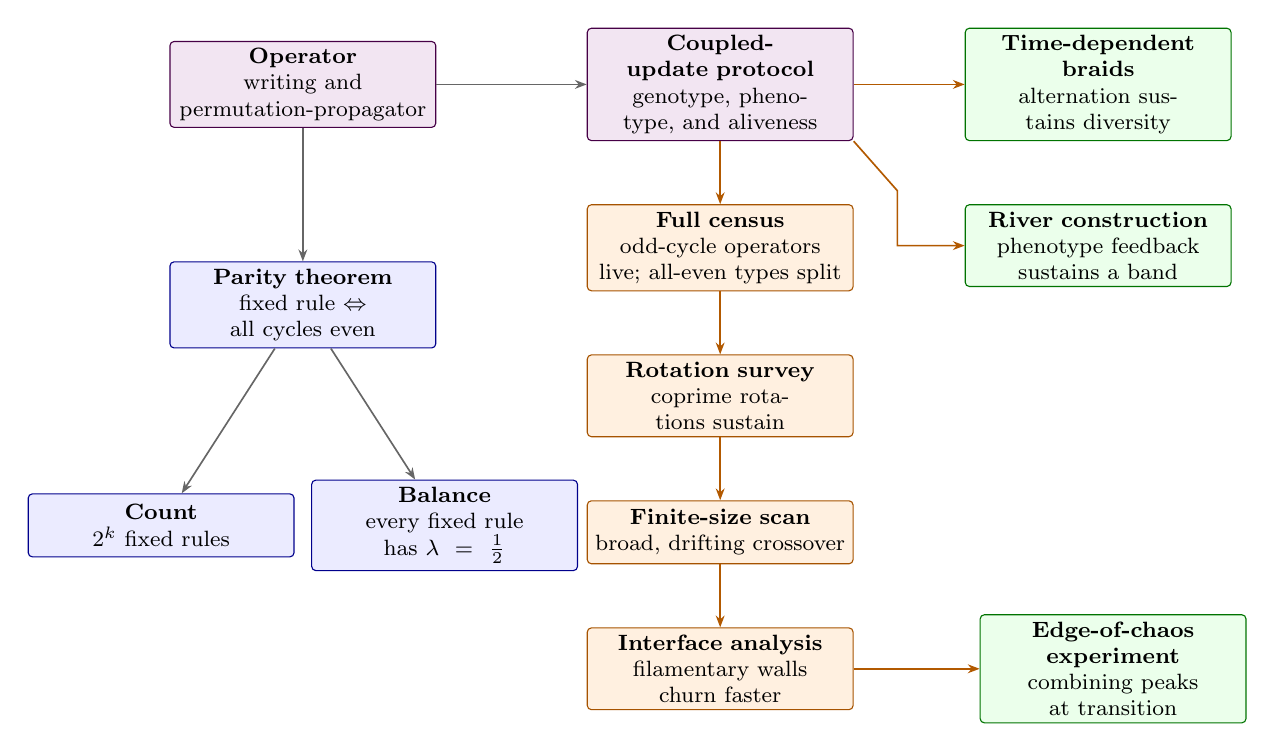
\begin{tikzpicture}[font=\footnotesize, >={Stealth[length=1.5mm]},
  bx/.style={draw, rounded corners=1.5pt, align=center, inner sep=2.5pt,
             text width=32mm, minimum height=8mm},
  defn/.style={bx, fill=violet!10, draw=violet!55!black},
  thm/.style={bx, fill=blue!8, draw=blue!55!black},
  ef/.style={bx, fill=orange!12, draw=orange!65!black},
  con/.style={bx, fill=green!8, draw=green!45!black},
  s/.style={->, draw=black!60, semithick},
  e/.style={->, draw=orange!70!black, semithick}]
% Exact branch (left).
\node[defn] (operator) at (0,0) {\textbf{Operator}\\writing and permutation-propagator};
\node[thm] (parity) at (0,-2.8) {\textbf{Parity theorem}\\fixed rule $\Leftrightarrow$ all cycles even};
\node[thm] (count) at (-1.8,-5.6) {\textbf{Count}\\$2^k$ fixed rules};
\node[thm] (balance) at (1.8,-5.6) {\textbf{Balance}\\every fixed rule has $\lambda=\tfrac12$};
% Empirical branch (centre).
\node[defn] (protocol) at (5.3,0) {\textbf{Coupled-update protocol}\\genotype, phenotype, and aliveness};
\node[ef,below=8mm of protocol] (census) {\textbf{Full census}\\odd-cycle operators live; all-even types split};
\node[ef,below=8mm of census] (survey) {\textbf{Rotation survey}\\coprime rotations sustain};
\node[ef,below=8mm of survey] (crossover) {\textbf{Finite-size scan}\\broad, drifting crossover};
\node[ef,below=8mm of crossover] (walls) {\textbf{Interface analysis}\\filamentary walls churn faster};
% Constructive branch (right).
\node[con] (braid) at (10.1,0) {\textbf{Time-dependent braids}\\alternation sustains diversity};
\node[con,below=8mm of braid] (river) {\textbf{River construction}\\phenotype feedback sustains a band};
\node[con,right=16mm of walls] (compute)
  {\textbf{Edge-of-chaos experiment}\\combining peaks at transition};
% Arrows show dependence, not merely reading order.
\draw[s] (operator)--(parity); \draw[s] (parity)--(count); \draw[s] (parity)--(balance);
\draw[e] (protocol)--(census); \draw[e] (census)--(survey);
\draw[e] (survey)--(crossover); \draw[e] (crossover)--(walls);
\draw[s] (operator)--(protocol);
\draw[e] (protocol.east)--(braid.west);
\draw[e] (protocol.south east)--(7.55,-1.35)|-(river.west);
\draw[e] (walls.east)--(compute.west);
\end{tikzpicture}
\caption{\textbf{Argument map.} The exact branch (blue) derives fixed-point
existence, number, and balance from the operator definition. The empirical
branch (amber) uses the coupled-update protocol to move from the full census to
the rotation survey, finite-size scan, and interface analysis. The forward
branch (green) tests two ways of sustaining structure and a sampled
edge-of-chaos computation experiment. Arrows mark logical or methodological
dependence; figures visualise the corresponding measurements but are not
themselves premises.}
\label{fig:map}
\end{figure}

Box~\ref{box:propagator} works through one member of the
family bit by bit.

\begin{workedexample}[label={box:propagator}]{A simultaneous propagator by hand}
\small
Write an ECA rule in Wolfram's standard neighbourhood order:
\begin{center}
\setlength{\tabcolsep}{3.2pt}
\begin{tabular}{c@{\quad}*{8}{c}}
position & $0$ & $1$ & $2$ & $3$ & $4$ & $5$ & $6$ & $7$ \\
neighbourhood & $111$ & $110$ & $101$ & $100$ & $011$ & $010$ & $001$ & $000$ \\
\midrule
Rule 110 & $0$ & $1$ & $1$ & $0$ & $1$ & $1$ & $1$ & $0$ \\
\end{tabular}
\end{center}
Thus Rule~110 is the byte $01101110$. Let $\sig(p)=p+2\pmod 8$ on the
displayed position indices: each source bit is complemented and written two
positions further to the right, wrapping at the end.
Carrying out the eight writes gives
\[
P_{+2}(01101110)=01100100,
\]
which is Rule~100. This changes what the cell does to its black-and-white
phenotype. For example, neighbourhood $011$ maps to $1$ under Rule~110 but
to $0$ under Rule~100. The propagator has not directly flipped a phenotype
cell; it has changed the truth table that the cell will use.
\end{workedexample}

The simultaneous operator acts on one eight-bit rule; the spatial experiments
place its elementary writes inside a two-layer automaton.

\begin{definition}[Genotype and phenotype]\label{def:genopheno}
Each cell carries an eight-bit rule. The field of rules---the
\emph{genotype}---governs a field of black-and-white states---the
\emph{phenotype}---and neighbouring rules also interact. One complete local
update (Box~\ref{box:metaca-step}) evolves both layers; this is the computation
behind the space--time diagrams in Figure~\ref{fig:regimes}.
\end{definition}

\Needspace{0.72\textheight}
\begin{workedexample}[label={box:metaca-step}]{One site, one complete MetaCA step}
\small
At time $t$, site $x$ holds an eight-bit rule $g_x(t)$ and a phenotype bit
$X_x(t)$. One ordinary coupled step has three parts.
\begin{enumerate}
\item \textbf{Express the current rule.} The phenotype neighbourhood is
evaluated by the rule at its centre. With numerical neighbourhood value
$n_x(t)=4X_{x-1}(t)+2X_x(t)+X_{x+1}(t)$, its displayed position is $7-n_x(t)$:
\[
X_x(t+1)=g_x(t)\bigl(7-n_x(t)\bigr).
\]
\item \textbf{Blend neighbouring rules.} For each truth-table position $j$,
inspect the three genotype bits
$\bigl(g_{x-1}(j),g_x(j),g_{x+1}(j)\bigr)$. If the two outer bits agree, copy
their value. Thus $(0,1,0)$ blends to $0$. If they disagree, the centre rule
decides by treating the triple as one of its ECA neighbourhoods, converting
its numerical value $n$ to displayed position $7-n$ as above. The eight
coordinate-wise decisions form an intermediate rule
\[
h_x=B\bigl(g_{x-1}(t),g_x(t),g_{x+1}(t)\bigr).
\]
\item \textbf{Write one propagated bit.} Draw a source position
$K_x(t)\in\{0,\ldots,7\}$ uniformly and apply its elementary write to the
intermediate byte:
\[
g_x(t+1)=U_{\sig,K_x(t)}(h_x).
\]
\end{enumerate}
The ordinary spatial runs make one such elementary write per cell and
generation. The historical Figure~8 variant made two. By contrast,
$P_\sig$ denotes the simultaneous eight-write map classified in
\secref{sec:classification}; its fixed bytes are precisely the bytes left
unchanged by every possible elementary write.
\end{workedexample}

The substrate---a cellular automaton whose cells hold rules rather than
states---is not itself new \parencite{corneli2015search}; what we study
is the \emph{operator} of Equation~\eqref{eq:prop}, understood as an
enumerated, exactly classified family. That 2015 paper found a single
member of this family, encountered through a programming error and not
recognised as one of many; we now give the family an essentially complete
characterisation. The canonical symmetry group of ECA
rule space has order four (reflection $\times$ complement, collapsing $256$
rules to $88$ classes) \parencite{svozil2025symmetries}; it is not $S_8$,
and the negation-carrying, $\sig$-parameterised family of
Equation~\eqref{eq:prop} does not appear in it. Rule-space permutation as a
parameterised, enumerated family with a derived fixed-point structure does
not appear in the literature we have surveyed; the nearest neighbours
augment cellular automata with state-dependent feedback
\parencite{pavlic2014selfref} rather than permuting the rule itself. Two
established genres are adjacent but distinct: per-cell rules (non-uniform or
$\nu$-CA \parencite{dennunzio2011nonuniform}) and rules that change during
evolution (rule-changing or programmable CA
\parencite{mori1998rulechanging}). Non-uniform cellular automata are not, by
themselves, the source of novelty here: when each site draws its rule from a
finite set, the resulting system can be represented as a uniform cellular
automaton on a product alphabet \parencite{dennunzio2011nonuniform}. Our
contribution instead concerns the permutation-propagator family and its
fixed-point structure.

\begin{figure}[tp]
\centering
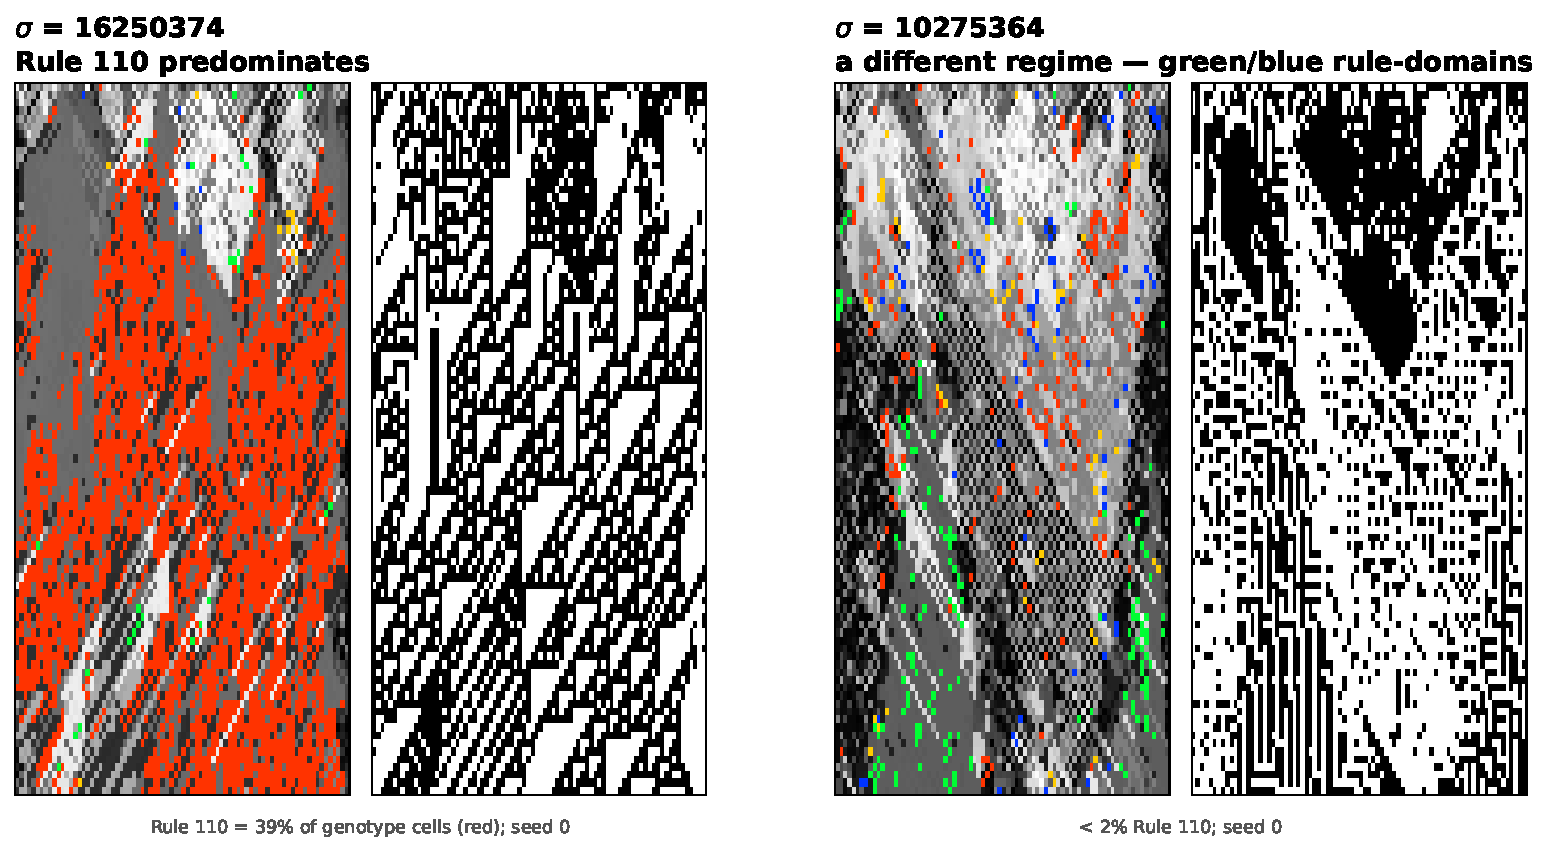
\includegraphics[width=\linewidth]{figures/rule110_spread.pdf}
\caption{Two operators from the family, each shown over time as genotype
(256-colour, left) and phenotype (black and white, right). Under
$\sig = 16250374$ the genotype field comes to be dominated by ECA
Rule~110---the red cells, $39\%$ of the genotype at the representative seed
($35\%$ over six seeds)---and the phenotype accordingly displays Rule~110's
characteristic gliders; under $\sig = 10275364$ a different regime of
rule-domains forms (green and blue, under $2\%$ Rule~110). The operator does not merely stir rule space: it
drives it toward particular, computationally distinguished rules. Genotype
colours are the legacy engine's own.}
\label{fig:regimes}
\end{figure}

\section{The Classification}
\label{sec:classification}

\subsection{Fixed points exist iff every cycle is even}

\begin{theorem}\label{thm:parity}
$P_\sig$ has a fixed point (a fixed rule) if and only if every cycle of
$\sig$ has even length. Since a one-cycle has odd length, this already
requires $\sig$ to be fixed-point-free.
\end{theorem}

\noindent A fixed rule is a $g$ invariant under~\eqref{eq:prop}, i.e.\ a
$\sig$-equivariant Boolean colouring with $g(\sig k) = \lnot\,g(k)$.
Follow a cycle of length $L$: equivariance forces
$g(k) = (\lnot)^{L} g(k)$, and $(\lnot)^{L}$ is the identity exactly when
$L$ is even; conversely, colour each orbit by the parity of its distance
from a chosen representative. A one-cycle of $\sig$ ($L=1$) is odd and so
admits no such colouring, which is why even cycles are required throughout.

Box~\ref{box:even-cycle} shows the theorem on the offset-$+2$ operator. The
same small calculation also makes the later $2^k$ count and forced
$\lambda=1/2$ balance visible before we state them generally.

\begin{workedexample}[label={box:even-cycle}]{Even and odd cycles}
\small
For offset $+2$ on eight truth-table positions,
\[
\sig=(0\;2\;4\;6)(1\;3\;5\;7).
\]
A fixed rule must change colour at every arrow because
$g(\sig k)=\lnot g(k)$. Around either four-cycle it can therefore read
$0101$ or $1010$: after four negations it returns consistently to its
starting bit. The two four-cycles are coloured independently, so two binary
choices fix all eight truth-table entries $\bit{0},\dots,\bit{7}$. Read back as
an ECA rule number---those eight bits in Wolfram neighbourhood order (the table
of \secref{sec:object}) taken as an integer in $0$--$255$---the four colourings
are the fixed rules
\[
2^2=4:\quad
51,\ 102,\ 153,\ 204,
\]
each with four zero-bits and four one-bits. An odd cycle admits no such
colouring: after an odd number of negations the bit returns to its starting
position demanding its own opposite, so no fixed rule exists. Admitting a fixed
rule and settling onto one are distinct. An operator carrying an odd cycle has no
fixed rule for its field to collapse onto, and its field correspondingly stays
diverse (the any-odd reduced rotate$+2$, Figure~\ref{fig:parity}, right); whether
a fixed-point-bearing operator collapses onto one of its fixed rules is a
separate, dynamical question (\secref{sec:interrupter}).
\end{workedexample}

This is the signed-cycle fixed-point theorem of Boolean-network theory
\parencite{aracena2008maximum} specialised to~\eqref{eq:prop}: our operator
is a Boolean network whose signed interaction digraph is $\sig$ with every
arc negative, a negation-cycle of length $\ell$ has sign $(-1)^\ell$, and
an isolated negative cycle admits no fixed point while a positive (even)
one admits exactly two. We contribute a machine-checked proof of the
specialised statement in Lean~4 / Mathlib.\footnote{%
\texttt{DarkTower/Patterns/Propagator.lean}, theorem
\texttt{hasAlternatingColouring\_iff\_cycleType\_even}; \texttt{lake build}
clean, no \texttt{sorry} or \texttt{axiom}.}

\subsection{The closed form}

The number of $\sig \in S_{2n}$ with all cycles even is $((2n-1)!!)^2$, with
exponential generating function $\sum_n ((2n-1)!!)^2 x^{2n}/(2n)! =
1/\sqrt{1-x^2}$ (the ``set of even cycles'' construction).
For $S_8$ this is $105^2 = 11{,}025$ of $40{,}320$, or $27.34\%$. The count
is classical: it is \textcite{oeis_a001818} and appears as
\textcite[Problem~5.34(c)]{stanley1999enumerative} and in
\textcite{riordan1968combinatorial}. We claim it only as the enumeration of
our operator family, not as a new identity.

\subsection{Fixed bytes number \texorpdfstring{$2^k$}{2 to the k}}

\begin{corollary}\label{cor:count}
An all-even $\sig$ with $k$ cycles has exactly $2^k$ fixed bytes; any $\sig$ with
an odd cycle has none.
\end{corollary}
Each even cycle admits exactly two alternating colourings, chosen independently
across cycles, whence $2^k$; the zero case is Theorem~\ref{thm:parity}. This too
is machine-checked.%
\footnote{\texttt{alternatingColouring\_card\_eq\_two\_pow\_cycleType\_card}.}
Summed against these weights the family is consistent:
$\sum 2^{k}$ over all-even $\sig$ equals $(2n)! = 8! = 40{,}320$, the total
number of fixed bytes across the family.

\section{Every Fixed Point Is Balanced}
\label{sec:lambda}

\begin{definition}[Langton's activity $\lambda$]\label{def:lambda}
$\lambda$ measures a rule's \emph{activity}: the fraction of its neighbourhood
entries that map to the non-quiescent
state~\parencite{langton1990computation}---for an eight-bit ECA table, the
Hamming weight over eight, $\lambda = \lVert r \rVert_1 / 8$, from $0$ (every
neighbourhood dies) through $1/2$ to $1$. A rule with $\lambda = 1/2$ is
\emph{balanced}.
\end{definition}

\begin{observation}[label={obs:lambda}]{Balance is a truth-table property}
Langton's thesis was that complex behaviour concentrates near a critical
$\lambda$, shown most clearly for larger tables ($K=4$, $N=5$); for the
two-symbol, three-neighbour ECAs Langton is explicit that $\lambda$ only roughly
correlates with dynamics, and later work is
cautious~\parencite{mitchell1993revisiting}. Theorem~\ref{thm:lambda} below
concerns the \emph{value} $\lambda = 1/2$ itself---balance---which we keep
separate from any empirical claim about what it predicts dynamically.
\end{observation}

\subsection{Every fixed point has \texorpdfstring{$\lambda = 1/2$}{lambda = 1/2}}

\begin{theorem}\label{thm:lambda}
Every fixed point of every operator in the family has exactly four one-bits;
equivalently, Langton's activity parameter $\lambda = 4/8 = 1/2$.
\end{theorem}

\noindent By Theorem~\ref{thm:parity} each cycle has even length $2m$; an
alternating colouring assigns such a cycle exactly $m$ ones; summing over
cycles gives $(\sum L)/2 = 8/2 = 4$. Exhaustive enumeration confirms it:
across all $40{,}320$ operators and all their fixed points, every one has
Hamming weight four, with zero exceptions. The statement is machine-checked
for $\mathrm{Fin}\,8$.\footnote{%
\texttt{alternatingColouring\_true\_card\_eq\_four}: the true-cells and
false-cells are put in bijection by $\sig$, forcing each to number four.}

We are deliberate about the standing of this result. Langton's critical
value was obtained empirically, as a statistic over rule space
\parencite{langton1990computation}, and its status as an order parameter
was contested: \textcite{mitchell1993revisiting} refuted
\textcite{packard1988adaptation}'s specific genetic-algorithm clustering
claim, not the definition of $\lambda$, which survived as one axis among
others such as Wuensche's $Z$ \parencite{wuensche1999classifying}. There is
a folklore intuition for why $1/2$ is special --- binomial sampling variance
$\lambda(1-\lambda)$ is maximal there --- and it is not ours; and it has been
noted that $\lambda$ alone does not fix a rule's dynamical class, distinct
classes coexisting at a single value \parencite{sakai2002edge}. What
Theorem~\ref{thm:lambda} adds is narrower and firmer than any of these: under
the complementation in~\eqref{eq:prop} the value $1/2$ is \emph{forced} as an
algebraic matter, because any alternation-under-complement colouring is
balanced by parity. We claim balance, exactly; any connection of that
balance to dynamical behaviour we treat as interpretation, not as part of the
theorem.

\subsection{The cast: which rules survive, and how many}

Under an all-even $\sig$, the fixed points of $P_\sig$---the rules it maps to
themselves---number $2^k$, where $k$ is the number of cycles of $\sig$
(\secref{sec:classification}): each even cycle admits two alternating
colourings, chosen independently across cycles. In the spatial runs these are
the rules onto which the field is observed to settle. Every one has
$\lambda = 1/2$ (Theorem~\ref{thm:lambda}), so the observed terminal
population is a cast of \emph{distinct} rules---distinct truth tables---sharing
a \emph{single} activity.

The smallest nontrivial case of the count is a single cycle, $k = 1$: two
survivors. The 2015 paper's Figure~8 already exhibited a two-rule residual: a
random field of tens of distinct rules dies off to an alternating population of
just two, rules $42$ and $170$.
Fittingly, the programming error that produced the family is what pins its
residual at two---the erroneous mutation froze a bit, splitting the field
into the cells that can reach $42$ and those that can reach $170$---so the
phenomenon was on the page before the $2^k$ count explained it.

That die-off curve---the count of distinct rules present over time---is a
natural population-level companion to $\lambda$. Where $\lambda$ is a scalar
assigned to a single rule, this curve is a property of the whole field's
trajectory; and where $\lambda$ is uninformative here---every fixed point
sits at $1/2$---the curve still varies, because it measures the population
rather than the point. We use it cautiously, as an observable rather than an
established order parameter, to tell the rotations whose fields stay diverse
from those whose fields collapse (\secref{sec:interrupter},
Figure~\ref{fig:lambda}).

Diversity of the observed population and singularity of its activity thus
coexist; the metric measures we tried do not separate the two
(\secref{sec:metrics}).

\begin{figure}[t]
\centering
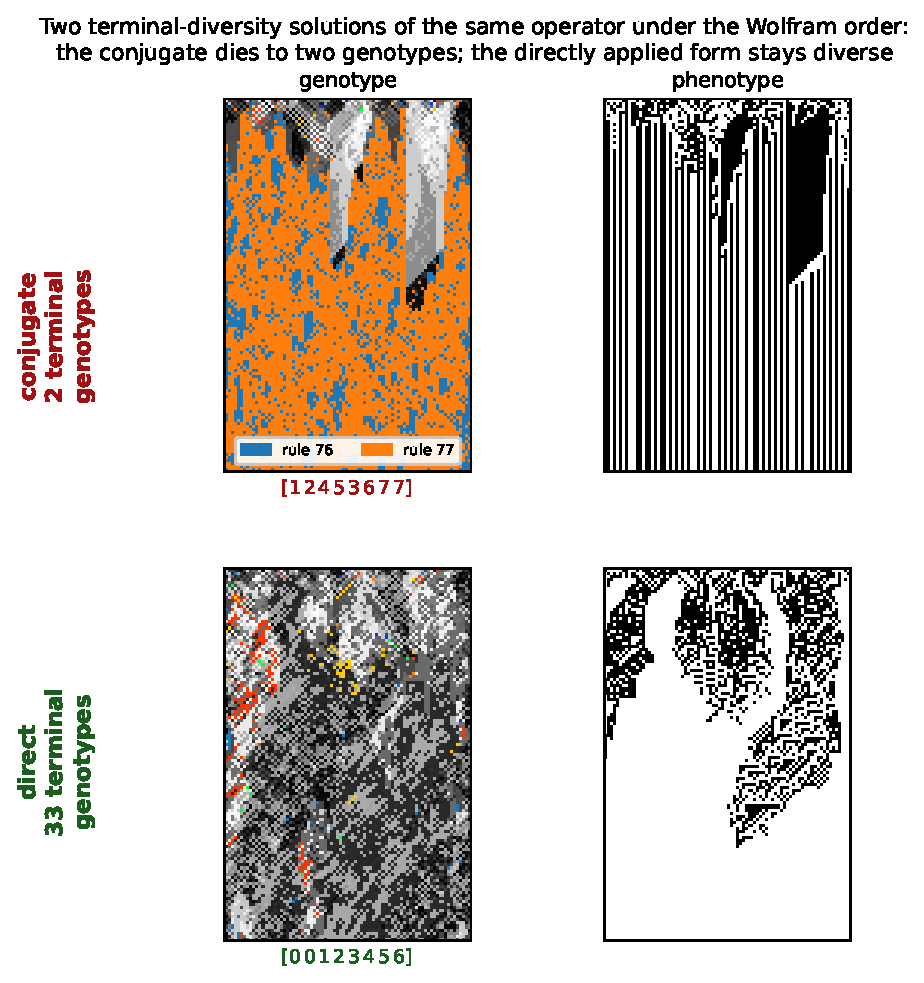
\includegraphics[width=0.82\linewidth]{figures/fig2pair.pdf}
\caption{\textbf{Two terminal-diversity solutions of one historical operator.} The
historical write $[0\,0\,1\,2\,3\,4\,5\,6]$ has two forms under the standard
Wolfram order. Its \emph{conjugate} $[1\,2\,4\,5\,3\,6\,7\,7]$ (top) reproduces the
two-rule behaviour: the genotype collapses to exactly two terminal rules---76 and 77,
adjacent, differing in a single bit---regardless of seed, while the phenotype stays
regular. Applied \emph{directly} (bottom), the same operator keeps a diverse
genotype (${\sim}30$ terminal rules). Two ends of genotypic
aliveness from one historical write.}
\label{fig:fig2pair}
\end{figure}

\subsection{A dead genotype can carry a live phenotype}
\label{sec:shell}

The balanced shell is a definite object: exactly $\binom{8}{4} = 70$ rules
carry four active outputs, and by Theorem~\ref{thm:lambda} the absorbing set of
every operator in the family lies wholly inside it. Collapse is therefore not
merely a loss of diversity but a fall onto this particular $70$-rule balanced
shell at $\lambda = 1/2$.

Balance is necessary for a genotype to freeze and silent about what the frozen
rule then does. Run each of the $70$ as an ordinary elementary CA and they
split: $32$ are phenotypically live---sustained change under iteration, the
additive rules $90$, $105$, $150$ and the class-IV rule $54$ among them---while
the rest fall quiescent. The two halves share a single $\lambda$; this is,
inside our family and by construction rather than by survey, the coexistence of
dynamical classes at one activity value that has long been urged against
$\lambda$ as an order parameter \parencite{sakai2002edge}. A field can thus die
in its genotype while the surviving rule keeps its phenotype in motion.

Figure~\ref{fig:shell} is such a field, built to specification. To seat a
collapse on a chosen live rule $R$ it suffices to pair $R$'s four active
positions with its four inactive ones as an involution: four transpositions, an
all-even operator that holds $R$ among its fixed points (Theorem~\ref{thm:parity}).
Whether the field actually settles onto that fixed rule is a separate, dynamical
question (as \secref{sec:interrupter} stresses); here it does. Carried out for
Rule~$54$ this yields
$\sig = [2\,3\,0\,1\,5\,4\,7\,6]$; run from a random field it drives the
genotype to near-uniformity---two rules survive---while the phenotype never
settles. The field has died onto Rule~$105$, another live tenant of the same
shell, whose additive dynamics keep the black-and-white panel full of
structure. Genotypic death and phenotypic death are not the same event.

One caveat marks the open edge of this. An involution fixes not its target
alone but the whole shell compatible with its pairing, and which tenant a
random field actually reaches is set by the basins, not by the construction: we
aimed at $54$ and the dynamics preferred $105$. Existence is settled---live
survivors are constructible---but \emph{steering} a field onto a named rule is
not, and is the natural next question.

\begin{figure}[t]
\centering
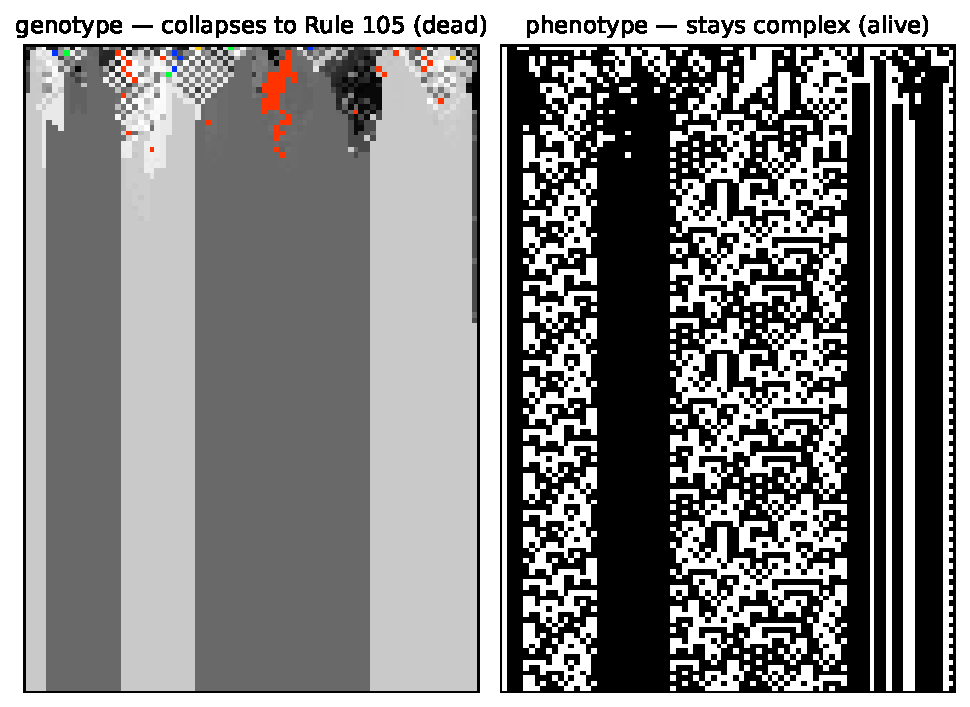
\includegraphics[width=0.82\linewidth]{figures/critical_shell.pdf}
\caption{A genotypically dead, phenotypically live field. The all-even operator
$\sig = [2\,3\,0\,1\,5\,4\,7\,6]$, built to fix the balanced shell containing
Rule~$105$, collapses the genotype (left, 256-colour) to near-uniformity within
a few dozen rows---two rules survive---yet the phenotype (right) never settles:
the field has died onto Rule~$105$, an additive $\lambda = 1/2$ rule whose
dynamics keep it complex. Seed~$1$, $W = 80$, $T = 120$.}
\label{fig:shell}
\end{figure}

\section{The Census}
\label{sec:census}

\subsection{The parity dichotomy in the spatial dynamics}

Theorems~\ref{thm:parity}--\ref{thm:lambda} concern fixed bytes; the spatial
dynamics adds stochastic elementary writes and, in the census, neighbour
blending. Figure~\ref{fig:parity} shows why fixed-point existence is not itself
a dynamical verdict: without blending, all-even rotate$+2$ settles within the
run while all-even rotate$+1$ remains diverse; the odd-cycle examples, which
lack fixed bytes, also remain diverse. The full census below
(\secref{sec:full-census}) makes this quantitative over all $40{,}320$ operators
(Table~\ref{tab:census}); the dynamical content is the \emph{death-rate
difference} between the classes, not the class sizes.

\begin{figure}[t]
\centering
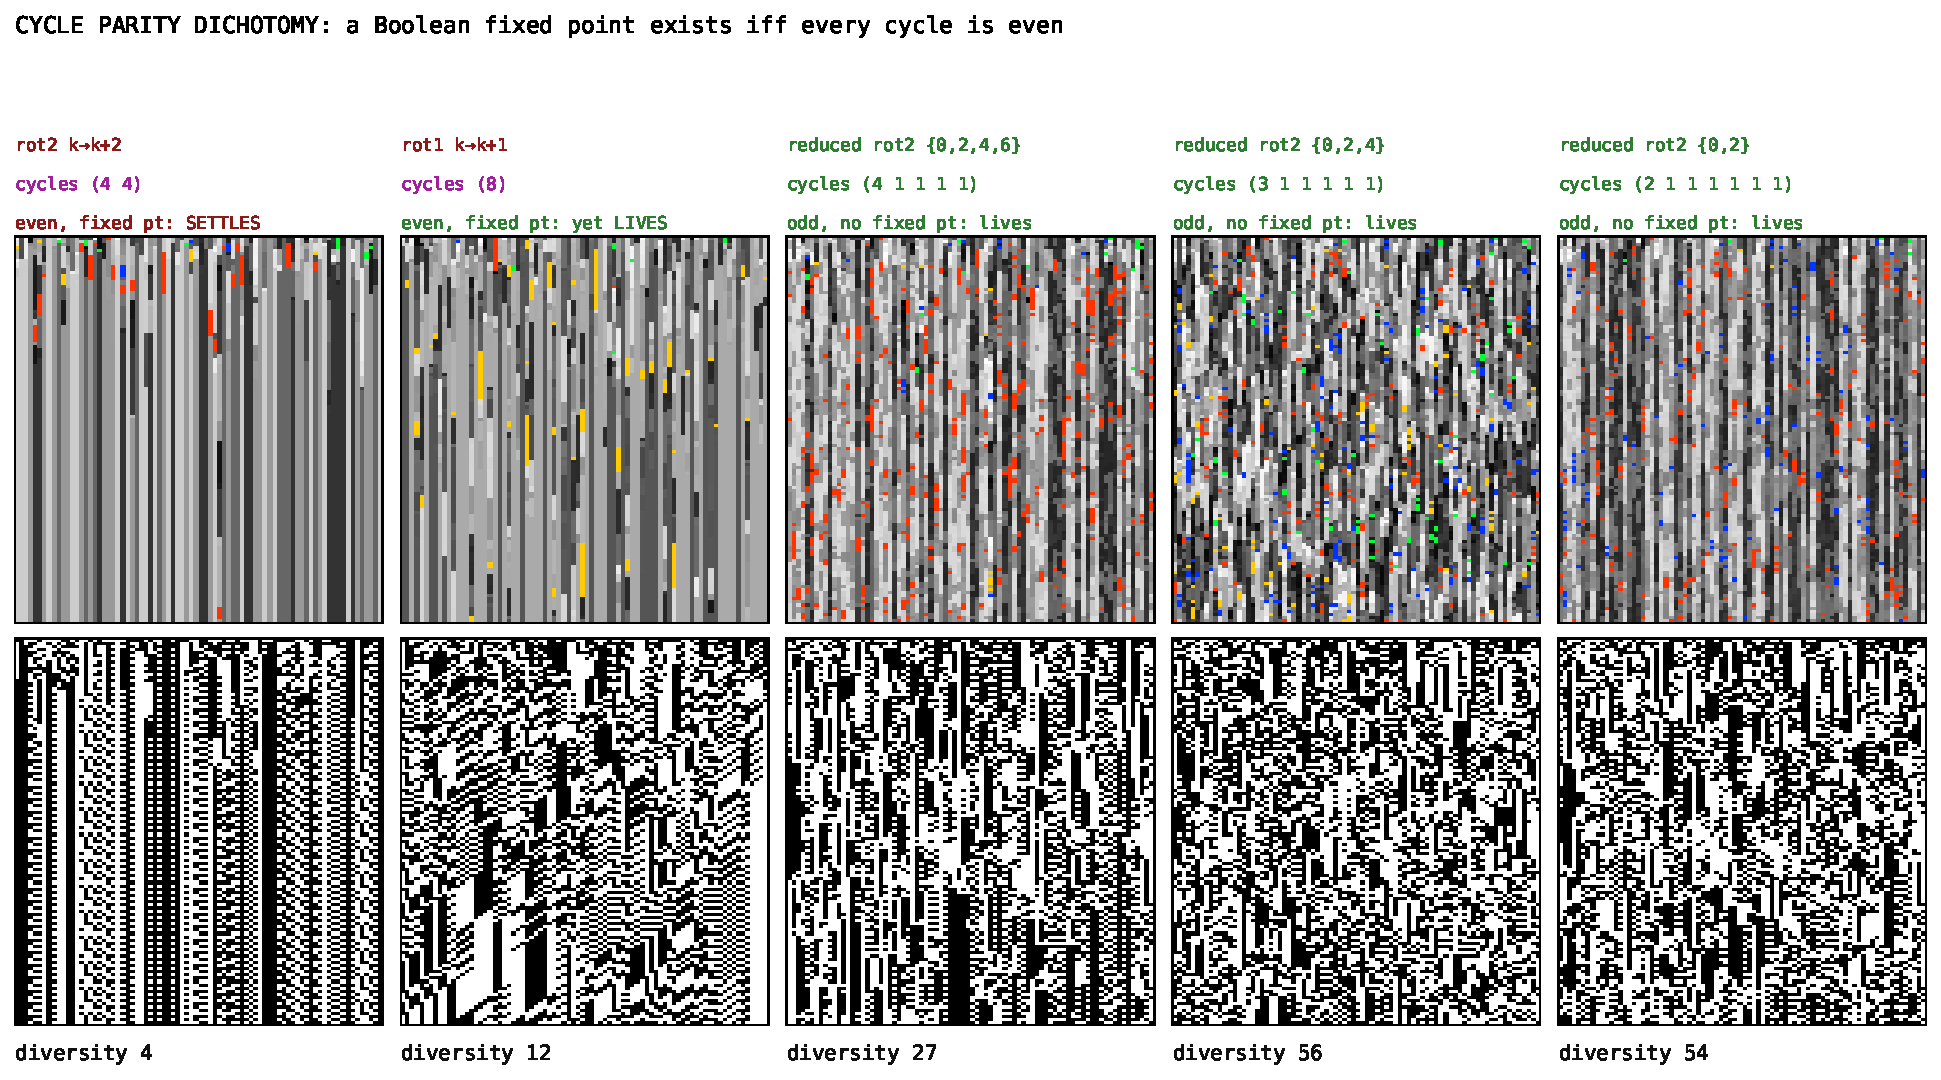
\includegraphics[width=\linewidth]{figures/parity-dichotomy.pdf}
\caption{The parity dichotomy, by example (the census of all $40{,}320$
permutations is summarised in the text). Five operators as genotype (top) and
phenotype (bottom) over time. \emph{Left:} both all-even operators possess fixed
bytes (Theorem~\ref{thm:parity}), but only rotate$+2$ settles within the run,
reaching its $2^k=2^2$ fixed rules; the single-8-cycle rotate$+1$ remains active
at diversity $12$. \emph{Right:} the odd-cycle operators
(reduced rotate$+2$, acting on a subset so the remaining positions are odd
one-cycles) possess no fixed byte and stay diverse in these runs. All five use
stochastic elementary writes without neighbour blending. The figure therefore
illustrates the theorem's fixed-byte classification while also showing that
all-even parity makes settling possible, not inevitable on a finite horizon.}
\label{fig:parity}
\end{figure}

\subsection{A prospective test: reduced \texorpdfstring{rotate$+2$}{rotate+2}}

To guard against reading structure into a completed enumeration, we fixed a
prediction before running the case. The reduced $\text{rotate}{+}2$
operators act as a single even cycle on a subset of positions and leave the
remaining positions as one-cycles; by that leftover they are \emph{not}
all-even, so by Theorem~\ref{thm:parity} they possess no fixed point and
should fall on the no-fixed-points side of the dichotomy---no rule for the
field to settle onto, and correspondingly less extinction. They do
(Figure~\ref{fig:parity}, right): they stay diverse rather than dying off.
Absence of fixed points forbids settling onto a single rule; it does not
forbid short-period behaviour, and we claim only the observed persistence of
diversity, not literal aperiodicity.

\subsection{The full census, tabulated by class}
\label{sec:full-census}

\begin{definition}[Census protocol and aliveness]\label{def:aliveness}
For each of the $40{,}320$ permutations, we ran seeds $0$--$2$ on a width-$60$
line for $100$ generations. Initial rule bytes are independent uniform draws
from $0$--$255$, initial phenotype bits are independent fair binary draws, and
both layers have fixed zero boundaries. Each genotype update uses the
neighbour blend and one uniformly sampled elementary write described in
Box~\ref{box:metaca-step}. A layer's \emph{change rate} is the mean fraction of
cells differing between consecutive rows over the final $40$ generations,
averaged over the three seeds. The layer is \emph{alive} when this rate is at
least $0.10$ and \emph{dead} otherwise. Scoring genotype and phenotype
separately gives four regimes: live/live, live/dead, dead/live, and dead/dead.
\end{definition}

The trend becomes an exhaustive finite-run observation once every operator is tabulated. We ran all
$40{,}320$ permutation-propagators and grouped them by cycle type
(Table~\ref{tab:census}).

\begin{empiricalfinding}[label={find:census}]{The full permutation census}
Every permutation containing an odd cycle lacks a fixed byte
(Theorem~\ref{thm:parity}); under the census protocol, all $29{,}295$ such
operators were classified genotype-alive. The theorem excludes a common fixed
byte for all elementary writes; the observed $100\%$ alive rate is an additional
dynamical result. Every all-even cycle type splits between live and dead
operators. Among those types, the alive fraction falls as the number of cycles
$k$ increases: $[8]$ ($k{=}1$) is $83\%$ alive, $[2\,6]$ and $[4\,4]$ ($k{=}2$)
$70$/$67\%$, $[2\,2\,4]$ ($k{=}3$) $49\%$, and $[2\,2\,2\,2]$ ($k{=}4$) $26\%$.
Overall, $92.5\%$ have a live genotype. The regime split is $82.7\%$ live/live,
$9.8\%$ live/dead, $6.0\%$ dead/dead, and $1.4\%$ dead/live, so all four regimes
occur among bijective operators.
\end{empiricalfinding}

\begin{table}[t]
\centering\small
\caption{Genotype-alive fraction by cycle type under the census protocol, over
all $40{,}320$ permutations. Any odd cycle forbids a fixed byte
(Theorem~\ref{thm:parity}); empirically, every such operator is alive. The
all-even types split, with collapse becoming more frequent as the number of
cycles $k$ increases.}
\label{tab:census}
\begin{tabular}{lrr}
\toprule
cycle type & count & genotype-alive \\
\midrule
any type with an odd cycle (17 types) & $29{,}295$ & $100.0\%$ \\
$[8]$        & $5{,}040$ & $82.9\%$ \\
$[2\,6]$     & $3{,}360$ & $70.0\%$ \\
$[4\,4]$     & $1{,}260$ & $66.7\%$ \\
$[2\,2\,4]$  & $1{,}260$ & $49.2\%$ \\
$[2\,2\,2\,2]$ & $105$   & $25.7\%$ \\
\bottomrule
\end{tabular}
\end{table}

\section{Fixed Points Are Not Attractors}
\label{sec:interrupter}

\begin{figure}[p]
\centering
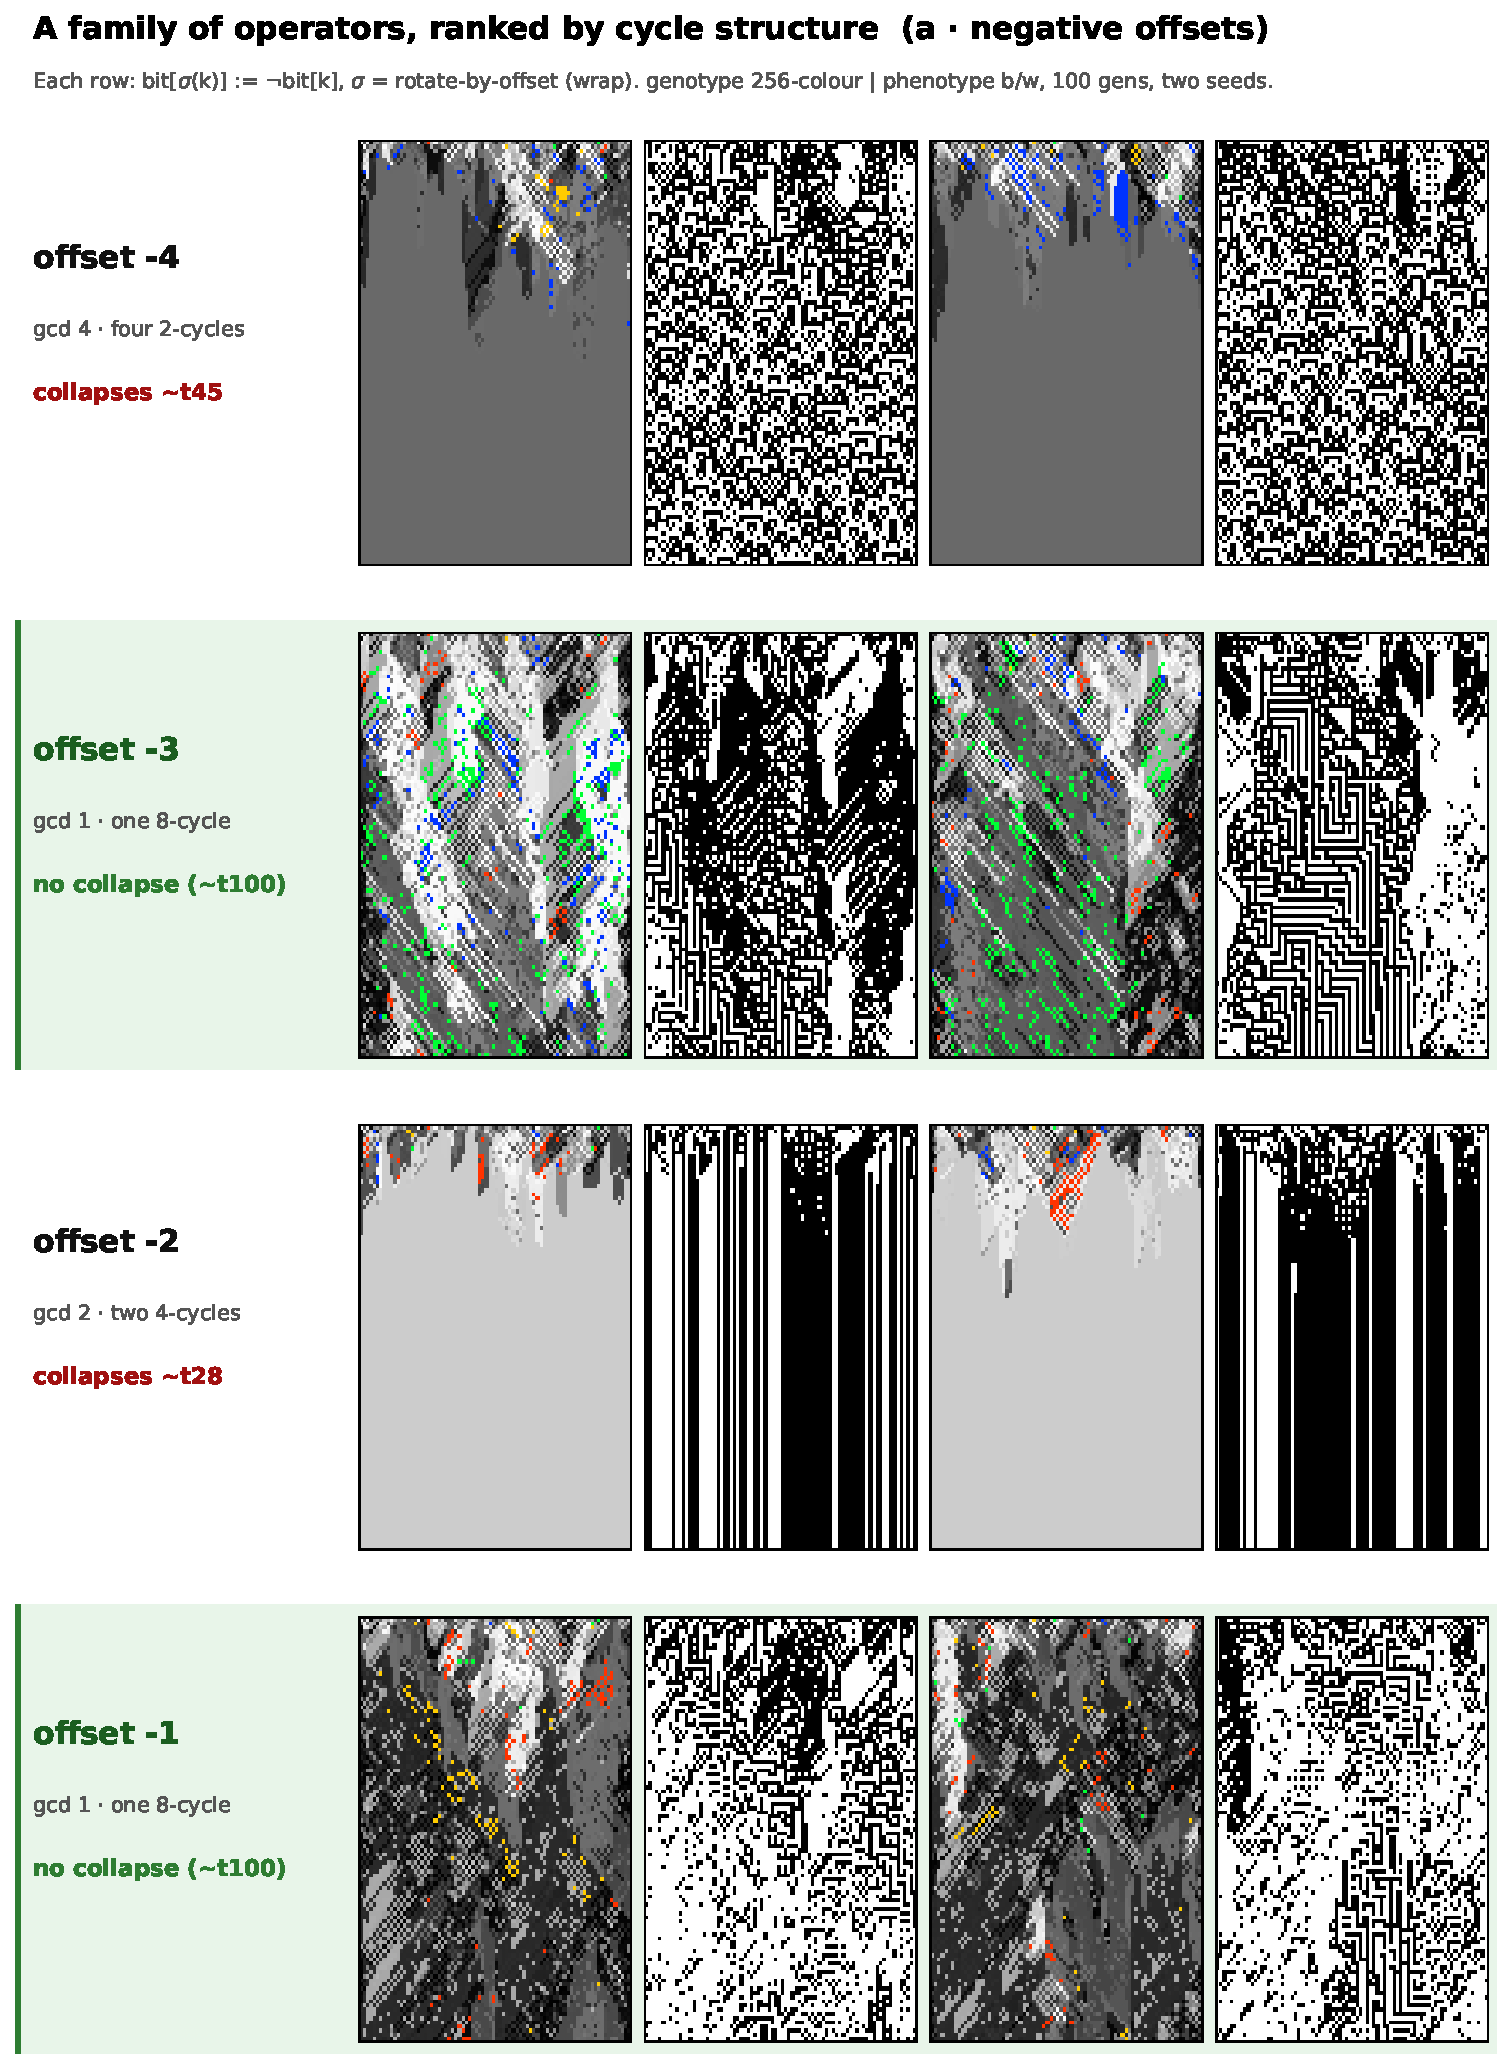
\includegraphics[height=0.73\textheight]{figures/survey_a.pdf}
\caption{\textbf{(a)~Negative offsets.} The rotation subfamily, ordered by
offset: each row is one wrap rotation $\bit{\sig(k)} := \lnot\,\bit{k}$ (two
seeds; genotype in 256 colours, phenotype black and white, first hundred
generations). Of these all-even rotations only the single 8-cycles,
$\gcd(\text{offset},8) = 1$---offset $\pm 1$ and $\pm 3$, highlighted---sustain a
high-diversity phase; offset $\pm 2$ ($\gcd 2$) and $\pm 4$ ($\gcd 4$) collapse.
See Worked Example~\ref{box:survey}; continued in~(b).}
\label{fig:eoc}
\end{figure}

\begin{figure}[p]
\ContinuedFloat
\centering
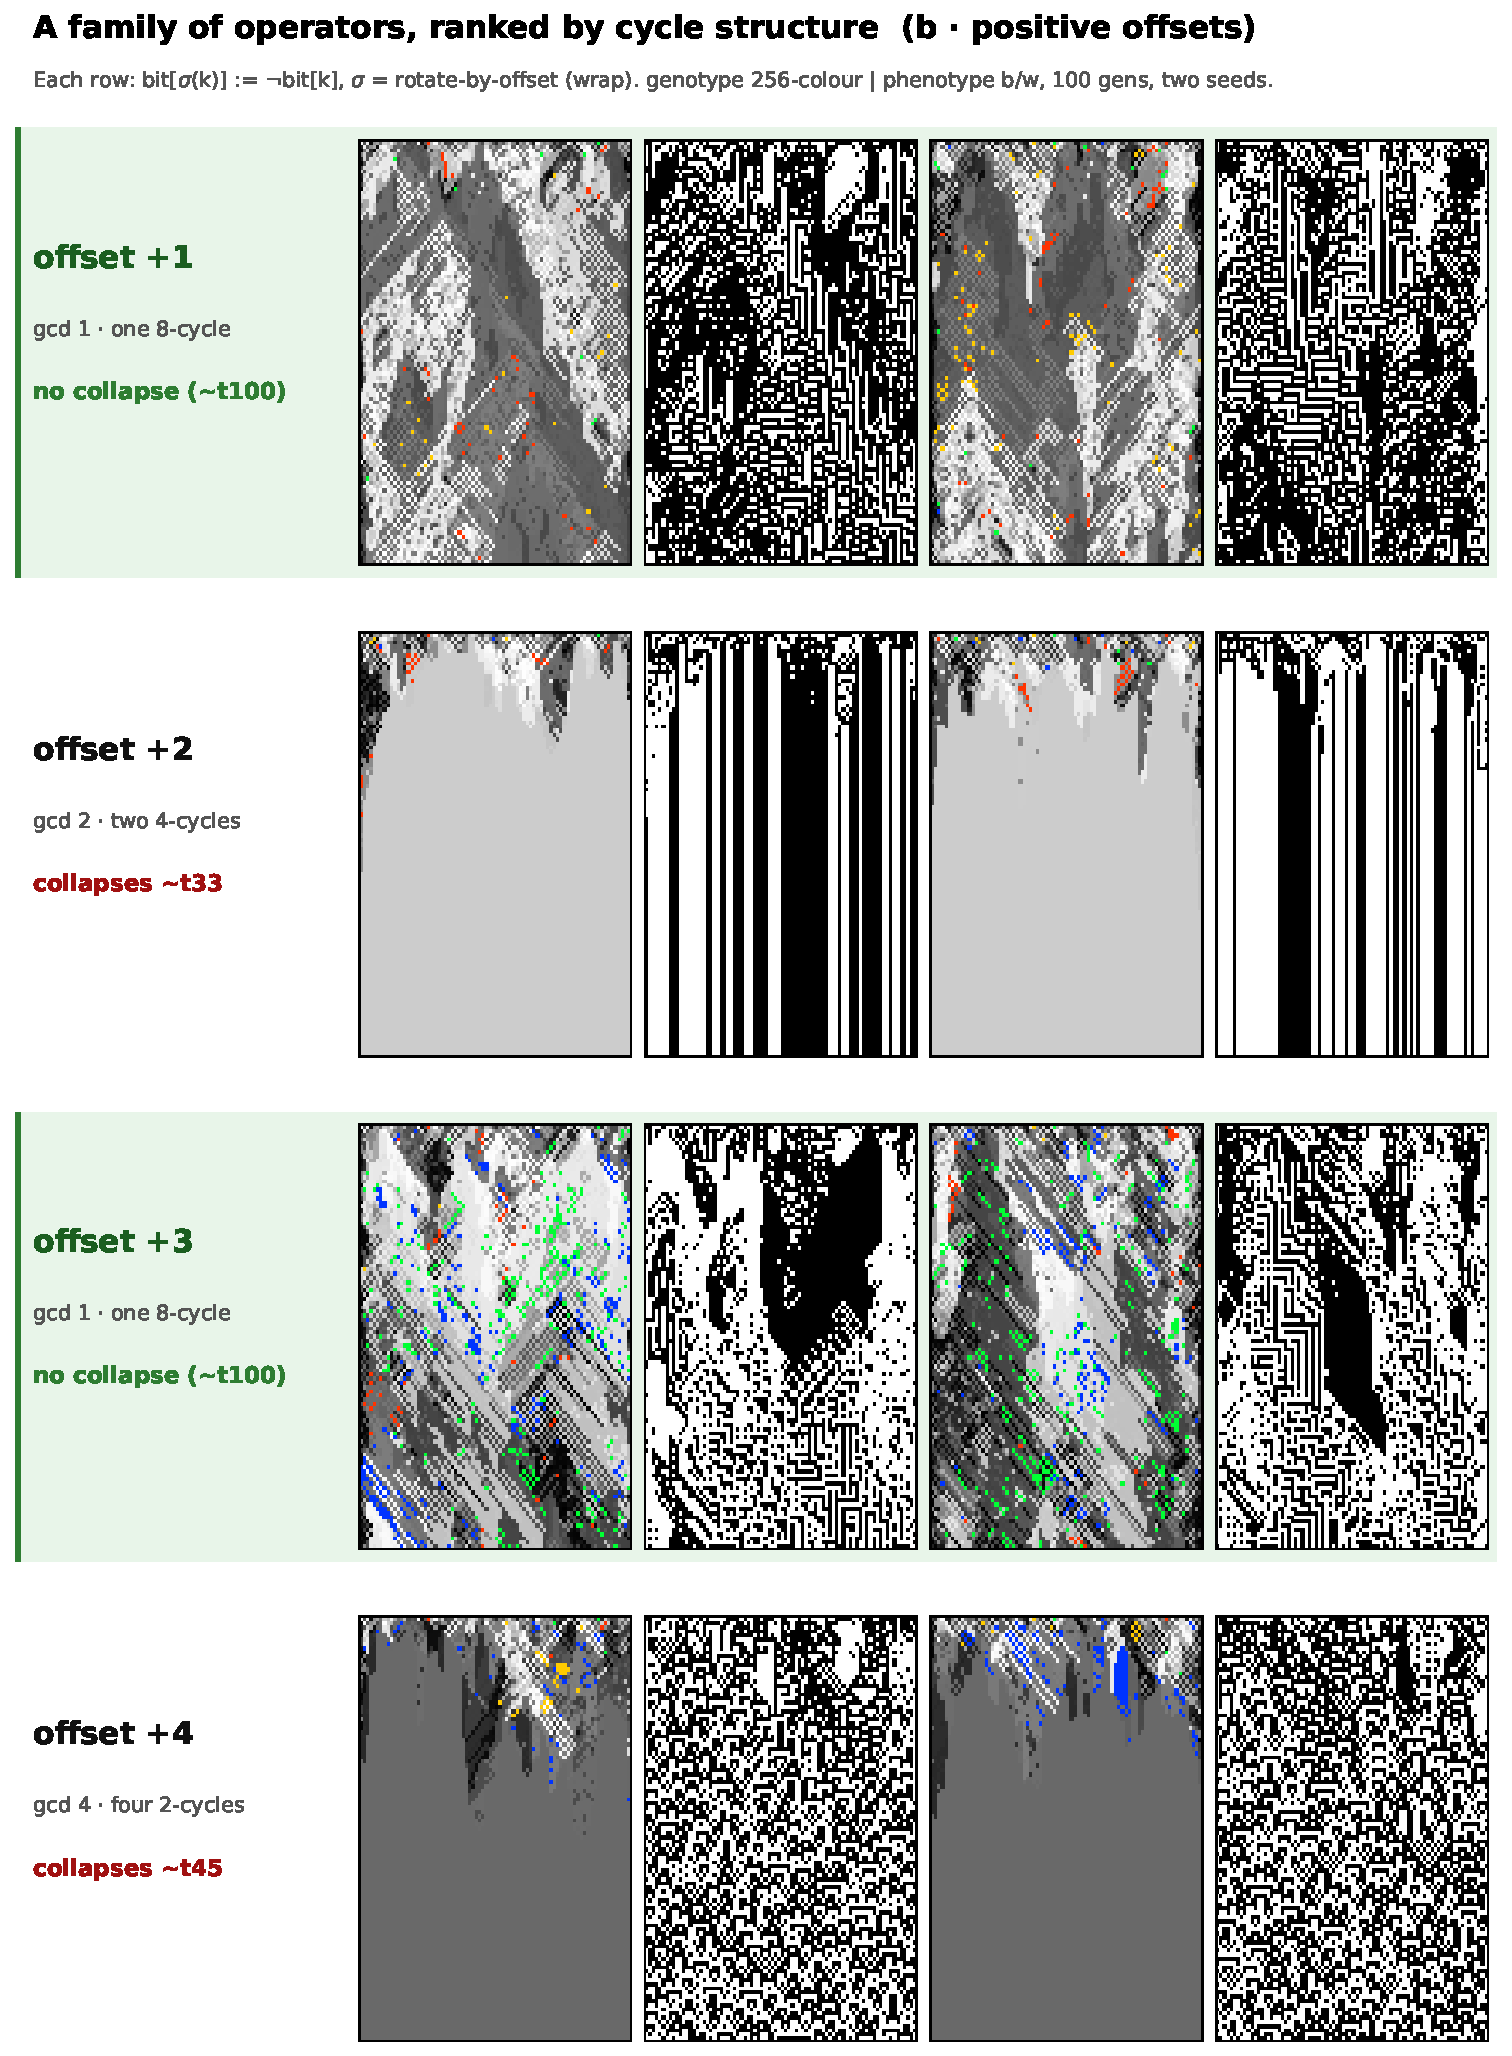
\includegraphics[height=0.73\textheight]{figures/survey_b.pdf}
\caption{\textbf{(b)~Positive offsets.} Continued from~(a). The classification is
symmetric under $d \to -d$ (verdict follows $\gcd(d,8)$), so offset $+1$ sustains
as offset $-1$ does, and offset $+2$ collapses as offset $-2$ does---inverse
rotations sharing verdict but not their transients (Worked
Example~\ref{box:survey}). Possessing a fixed point and staying near it are
different properties: the two pages visually summarise the distinction between
fixed-point existence and spatial persistence.}
\end{figure}

\begin{workedexample}[label={box:survey},breakable=false]{Reading the rotation survey}
\small
The fields of Figure~\ref{fig:eoc} evolve under the \emph{spatially coupled}
dynamics of \secref{sec:interrupter}---stochastic elementary writes together
with the coupling between cells---not $P_\sig$ applied cell-by-cell. This is
what the survey turns on. Without the blend, Figure~\ref{fig:parity} already
shows rotate$+1$ remaining active over the observed horizon while rotate$+2$
settles. With neighbour blending, the finite-horizon split persists and widens:
the single 8-cycles---$\gcd(\text{offset},8)=1$, offset $\pm 1$ and $\pm 3$---
sustain a high-diversity field, while offset $\pm 2$ ($\gcd 2$) and $\pm 4$
($\gcd 4$) collapse; that split is what the survey shows.

The two panels are \emph{almost} mirror images, and where they differ is
instructive. Offset $+d$ and offset $-d$ are the same permutation exactly when
$2d \equiv 0 \pmod 8$---so offset $\pm 4$ (and the identity) are one operator with
bit-identical panels, whereas offset $\pm 1$ and $\pm 3$ are distinct
\emph{inverse} rotations. Inverses share cycle structure, fixed rules, and the
sustain-or-collapse verdict, but not their transient dynamics: offset $+1$ and
offset $-1$ realise the same sustaining regime through visibly different fields.
\end{workedexample}

Possessing a fixed point (Theorem~\ref{thm:parity}) is not the same as
reaching one, and $P_\sig$ does not by itself move a rule toward
$\lambda = 1/2$. Because $P_\sig$ complements every bit,
$\lambda(P_\sig g) = 1 - \lambda(g)$: the operator \emph{reflects} activity
across $1/2$, exactly preserving the distance $\lvert\lambda - 1/2\rvert$
rather than contracting toward it. And because $P_\sig$ is a bijection on
bytes, a generic rule lies on a periodic orbit and simply cycles---its fixed
points are fixed, but they are not attractors and have no basins. The only
rules pinned at $\lambda = 1/2$ are the fixed points themselves. Attraction in
the experiments therefore belongs to the stochastic elementary-write dynamics,
with or without neighbour coupling, rather than to iteration of the simultaneous
map $P_\sig$.

\begin{empiricalfinding}[label={find:survey}]{The rotation survey}
Within the wrap-rotation subfamily, every non-trivial rotation is all-even and
so possesses fixed rules (Theorem~\ref{thm:parity}), yet under the
neighbour-blend coupling the tested rotations split by cycle structure
(Figures~\ref{fig:eoc},~\ref{fig:lambda}):
\begin{itemize}\setlength{\itemsep}{1pt}
\item the single 8-cycles---$\gcd(\text{offset},8)=1$, offset $\pm 1$ and
$\pm 3$---\emph{sustain} a high-diversity field, holding $\sim$30--40 distinct
rules through the longest runs we made ($400$ generations);
\item offset $\pm 2$ ($\gcd 2$, two $4$-cycles) and offset $\pm 4$ ($\gcd 4$,
four $2$-cycles) \emph{collapse} to one or two rules within a few dozen
generations.
\end{itemize}
The distinct-rule population curve (Figure~\ref{fig:lambda}) separates the two by
more than an order of magnitude in a single scalar. Possessing a fixed rule and
having the coupled field stay near it are different properties. The present
claim is limited to two seeds per rotation and treats population size as a
descriptive observable, not as an order parameter in the statistical-mechanics
sense.
\end{empiricalfinding}

\begin{figure}[t]
\centering
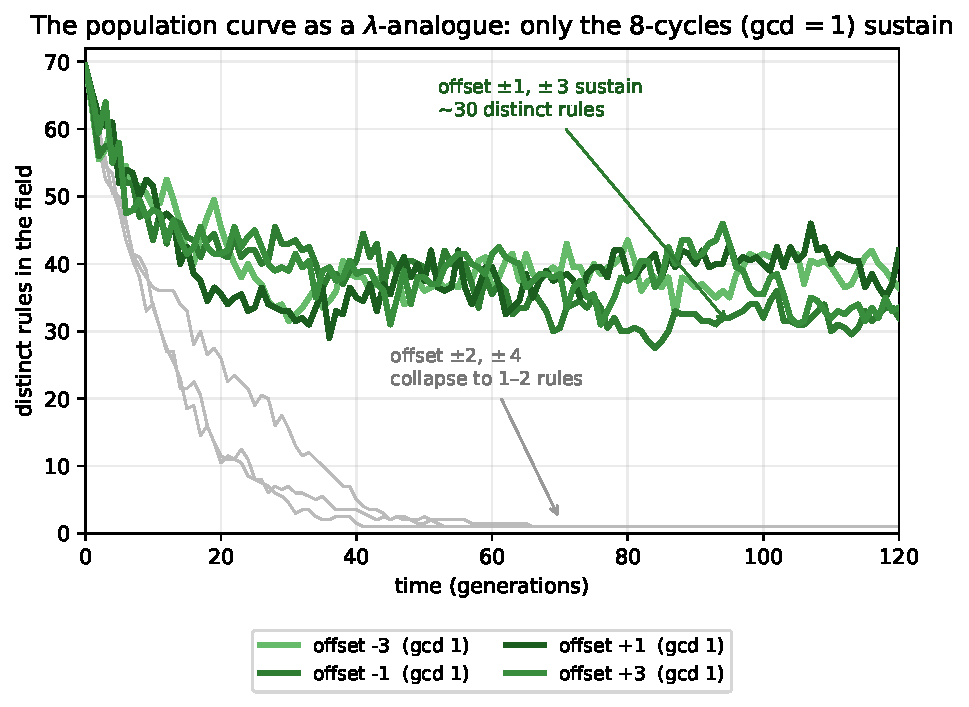
\includegraphics[width=\linewidth]{figures/lambda_analogue.pdf}
\caption{A population observable: distinct rules in the field over time, for
the wrap rotations (two seeds each). All begin at $\approx 70$; the four
8-cycles, $\gcd(\text{offset},8)=1$ (offset $\pm 1$ and $\pm 3$, green), keep a
large diverse population, while offset $\pm 2$ and $\pm 4$ (grey) collapse to one
or two rules. This makes quantitative, on the runs shown, the difference visible
by eye in Figure~\ref{fig:eoc}. Figure~\ref{fig:parity} gives the corresponding
without-blend comparison for offsets $+1$ and $+2$: the former remains active at
lower diversity over that run, while the latter settles onto its four fixed
rules.}
\label{fig:lambda}
\end{figure}

\begin{figure}[t]
\centering
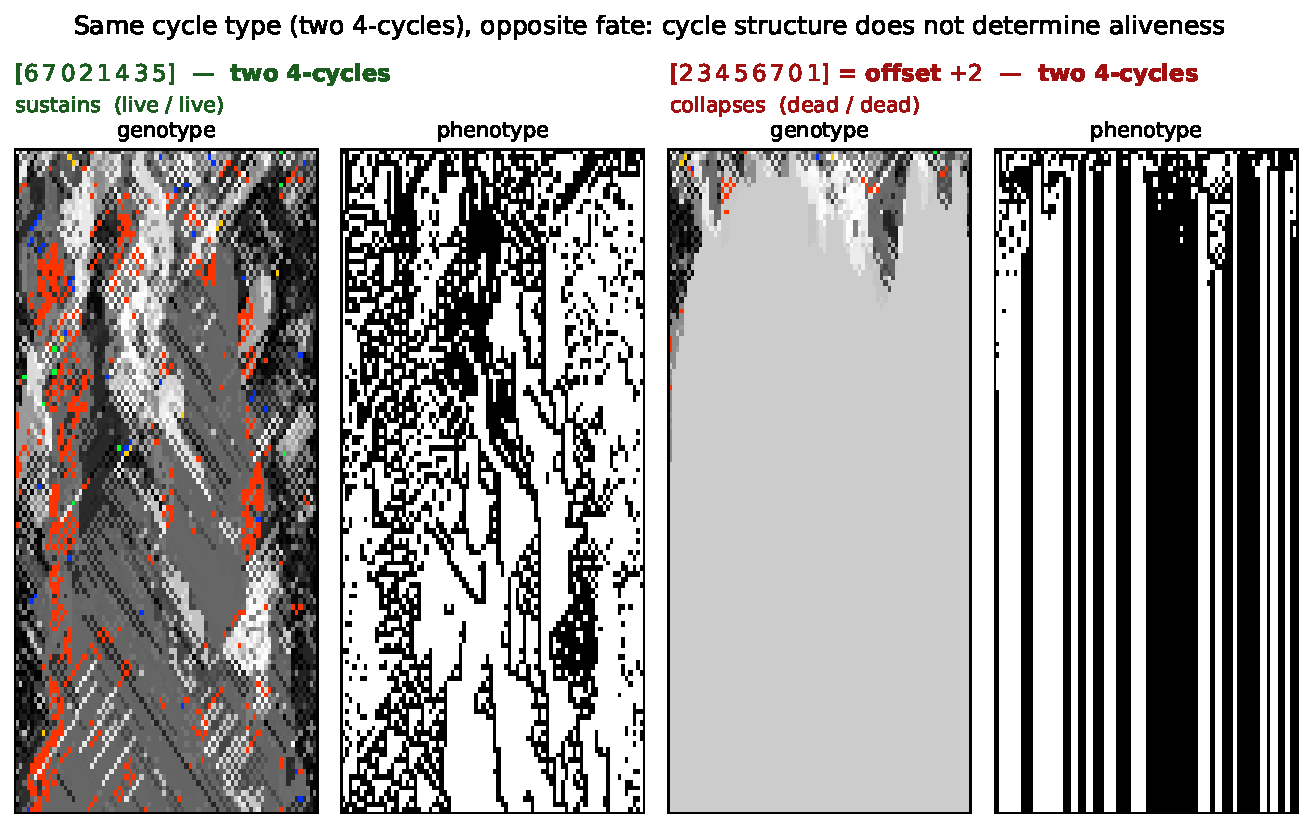
\includegraphics[width=\linewidth]{figures/two4cycle.pdf}
\caption{\textbf{Cycle structure does not determine aliveness.} Two operators of
identical cycle type---both two 4-cycles---with opposite fate. Left,
$[6\,7\,0\,2\,1\,4\,3\,5]$ sustains a live genotype and phenotype; it is the
standard-Wolfram-order form of the historical offset$+2$ operator (its
conjugate). Right, the Wolfram-order rotation offset$+2=[2\,3\,4\,5\,6\,7\,0\,1]$
has the same two-4-cycle structure yet collapses to a dead genotype and a frozen
phenotype. Same cycle type, opposite outcome: the specific permutation, not its
cycle type alone, decides. A full census of the 40320 operators confirms the
two-4-cycle class splits between sustaining and collapsing.}
\label{fig:two4cycle}
\end{figure}

\subsection{Constructive control by temporal schedules}
\label{sec:braiding}

\begin{definition}[Temporal braid]\label{def:braid}
A \emph{temporal braid} alternates two writings between complete coupled spatial
updates: writing $w_A$ is used at even times and $w_B$ at odd times. More
generally, a periodic \emph{schedule} selects one writing at each time step.
This preserves the intermediate spatial states and neighbour blends; it is not
the algebraic composition $P_{\sigma_A}\circ P_{\sigma_B}$ of two simultaneous
maps.
\end{definition}

\begin{empiricalfinding}[label={find:braid}]{A braid of two collapsing operators can sustain the field}
At width $80$, horizon $120$, and seed $0$, offset $+2$ and offset $+4$ each
have genotype change rate $0$ when held alone, while their alternating braid
has change rate $0.76$ (Figure~\ref{fig:braid}, top). The matched schedule
control offset $+2$/offset $-2$ remains dead (Figure~\ref{fig:braid}, bottom).
This establishes that two collapsing components can construct a sustaining
schedule. It does not establish the previously suggested block-system
criterion: all three even offsets preserve the evens/odds partition, and both
pairs generate the same translation subgroup $\langle {+2}\rangle$. The cause
of the contrasting braid outcomes remains to be identified.
\end{empiricalfinding}

\begin{figure}[t]
\centering
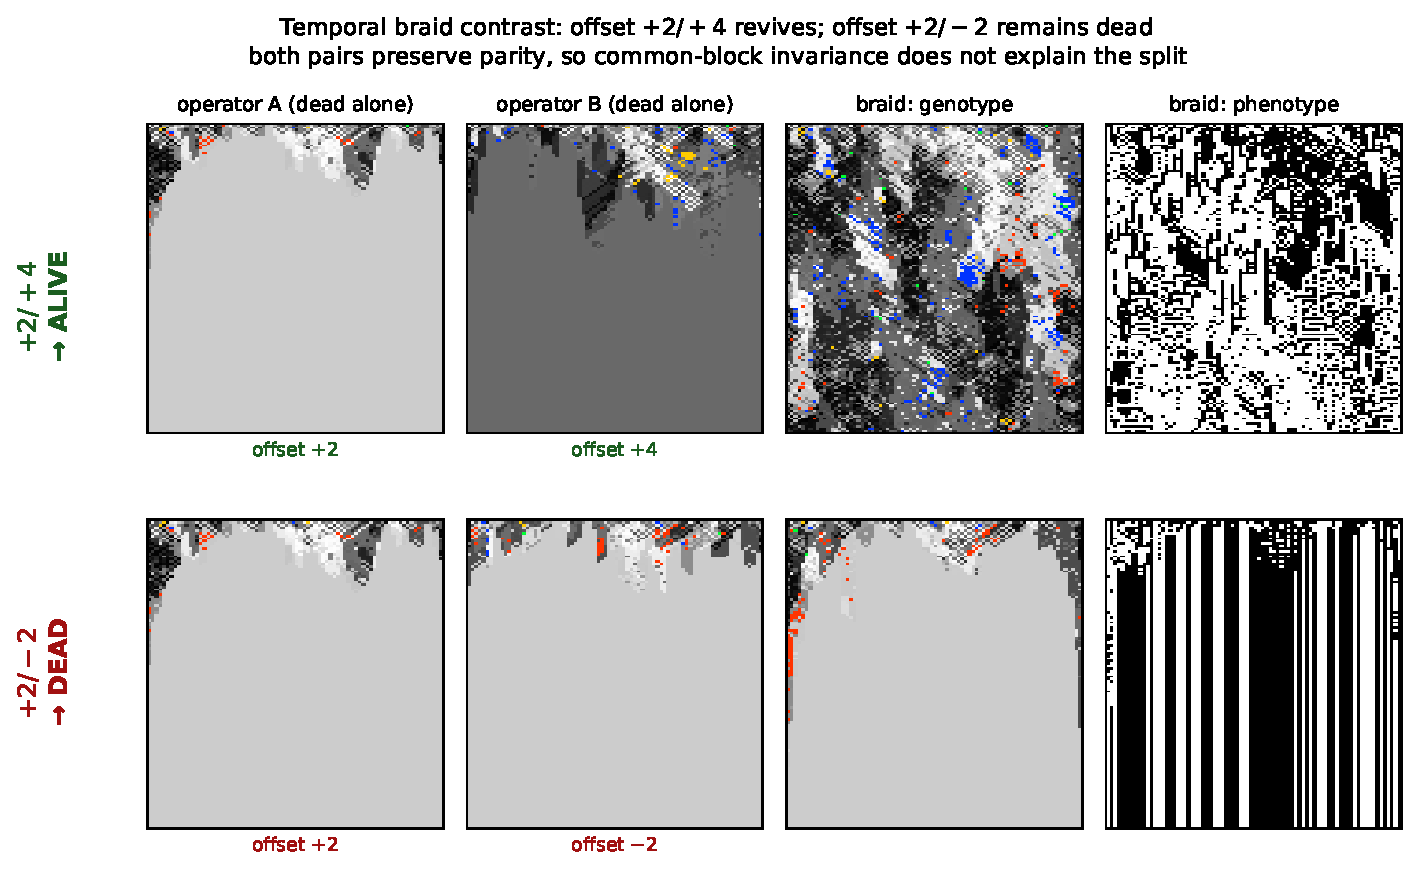
\includegraphics[width=\linewidth]{figures/braid.pdf}
\caption{\textbf{Temporal braiding can sustain aliveness.} Two operators that each collapse
alone are braided by alternating their elementary spatial updates. Top:
offset$+2$ (two
4-cycles) and offset$+4$ (four 2-cycles) are each genotypically dead, yet their
braid is alive (genotype change-rate $0.76$, vs.\ $0$ for either alone). Bottom:
offset$+2$ braided with offset$-2$ stays dead. Both tested pairs preserve parity,
so the contrast is not explained by the existence of that common invariant
partition. The result concerns time-dependent coupled dynamics, not composition
of the simultaneous maps $P_\sigma$.}
\label{fig:braid}
\end{figure}

\begin{empiricalfinding}[label={find:knob}]{The mixing fraction is a reproducible diversity control}
Let $\sigma$ be displayed-position offset $+1$. We ran periodic 12-step
schedules mixing the sustaining 8-cycle $\sigma^1$ with the collapsing
two-4-cycle operator $\sigma^2$, at width $80$ for $120$ generations and five
seeds per mixture. Mean late-window diversity rises from $1.0$ rule when the
$\sigma^1$ fraction is zero, through $16.8$ at fraction $0.25$, to $36.9$ at
fraction $5/12$; above that it remains in the range $34$--$41$ rather than
increasing monotonically (Figure~\ref{fig:knob}). The schedule fraction is thus
a tunable control for entry into a sustained high-diversity regime, with
saturation rather than a continuously linear response.
\end{empiricalfinding}

\begin{figure}[t]
\centering
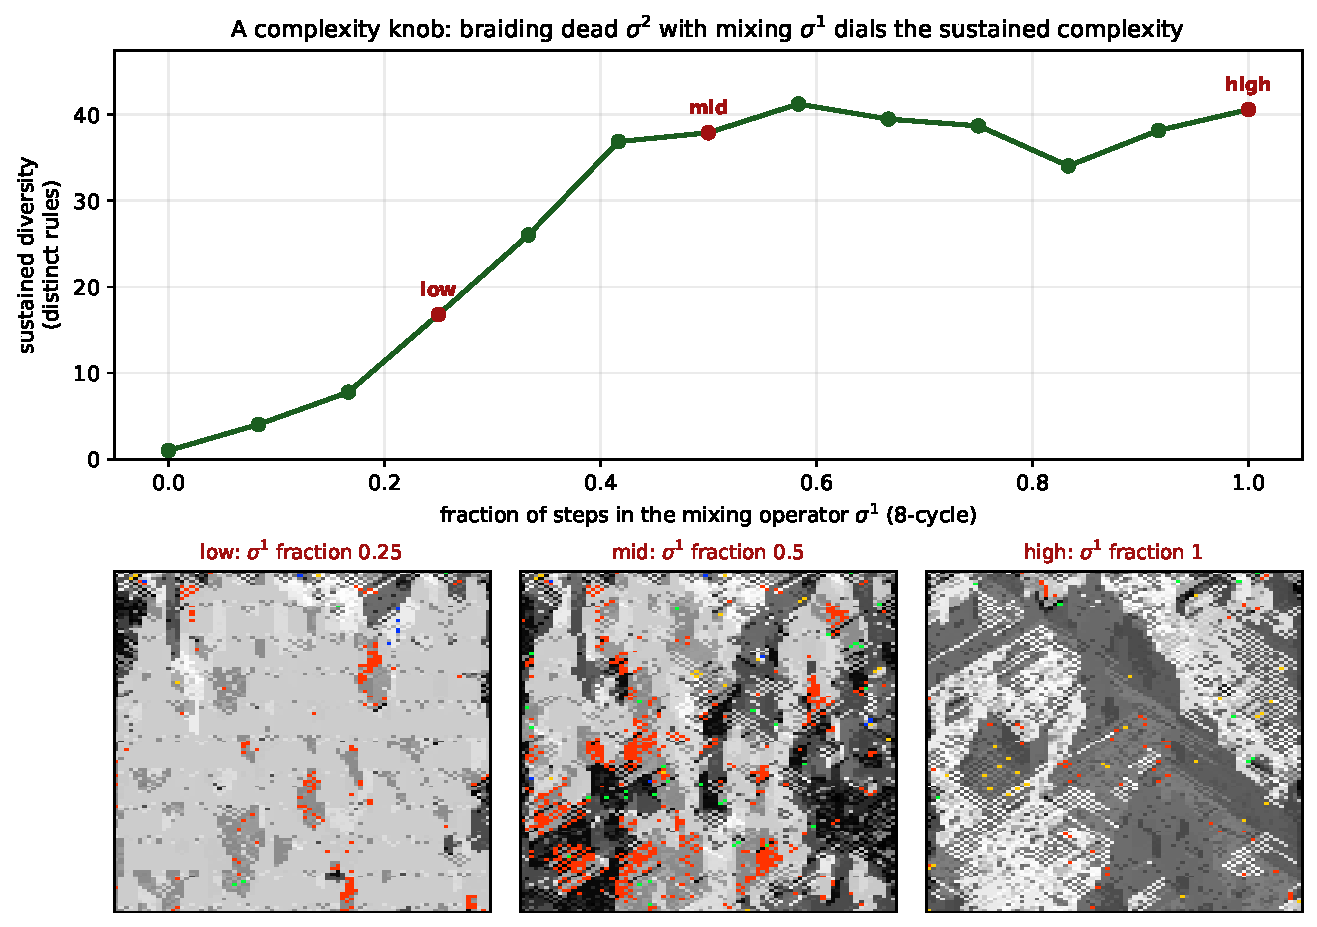
\includegraphics[width=\linewidth]{figures/knob.pdf}
\caption{\textbf{A diversity-control schedule.} Periodic 12-step schedules mix
the sustaining offset-$+1$ operator $\sigma^1$ with the collapsing offset-$+2$
operator $\sigma^2$. Mean late-window distinct-rule diversity (five seeds) rises
from $1.0$ with no $\sigma^1$ steps to a high-diversity plateau once its fraction
reaches roughly $0.4$. The three fields show fractions $0.25$, $0.50$, and $1.0$
at the same representative seed.}
\label{fig:knob}
\end{figure}

\begin{definition}[Interrupter]\label{def:interrupter}
An \emph{interrupter} is an update between elementary propagator writes that is
not itself a propagator write. The coordinate-wise neighbour blend of
Box~\ref{box:metaca-step} is the interrupter in the ordinary spatial runs; a
hold gate that suppresses a scheduled write is another example. An interrupter
changes the coupled dynamics but does not, by definition, guarantee sustained
diversity.
\end{definition}

\begin{empiricalfinding}[label={obs:couplings}]{The rotation split occurs with and without neighbour blending}
Figure~\ref{fig:parity} uses stochastic elementary writes without neighbour
blending; Figures~\ref{fig:eoc} and~\ref{fig:lambda} include the blend. Over the
displayed horizons, offset $+1$ remains active and offset $+2$ settles under
both protocols, although their diversity levels and transients differ. These
runs therefore do not identify neighbour blending as the cause of the split;
they show that fixed-byte existence alone does not determine finite-horizon
settling under either protocol.
\end{empiricalfinding}

\begin{proposition}[Composition parity]\label{obs:flat}
Products alternate between complemented and uncomplemented coordinate permutations.
Each operator of Equation~\eqref{eq:prop} negates every bit
($P_\sig(g)[j] = \lnot\,g[\sig^{-1}(j)]$, a coordinate permutation followed by a
global flip), so under composition the flips cancel in pairs: $P_\sig \circ
P_\tau$ is a \emph{pure} coordinate permutation with no negation left---a
bijection that fixes $2^{c}$ bytes for $c$ cycles but carries none of the forced
$\lambda = 1/2$ structure. An even number of propagators therefore composes to
an uncomplemented coordinate permutation, and an odd number to another member
of the permutation-propagator family.
\end{proposition}

Exploratory searches over products of two and three simultaneous propagators
found no additional structural regime. Temporal braiding is a different
operation: it alternates stochastic elementary writes inside the spatially
coupled dynamics rather than replacing them by one composed map.

Algebraic composition is therefore closed in the sense of
Proposition~\ref{obs:flat}. Temporal scheduling is different: it retains each
intermediate coupled state, which is why the braids of
\secref{sec:braiding} can produce dynamics absent from either held operator. A
second constructive mechanism pairs a propagator with a step of a different
kind.

\begin{definition}[River]\label{def:river}
A \emph{river} is the composed operator obtained by following the collapsing
offset-$+2$ propagator ($\gcd 2$) with a phenotype-reading construction
step---match the local phenotype against four template candidates, first match
wins, and fall back to the all-zero rule when none matches.
\end{definition}

\begin{empiricalfinding}[label={find:river}]{The river sustains a coherent band}
In all six tested seeds, the river produces a coherent band of alternating
phenotype that drifts through a disordered background
(Figure~\ref{fig:river}). Its trajectory varies with the seed, while its
presence persists for the full run. This is a six-seed observation, not a claim
that the structure is an attractor or survives arbitrarily long.
\end{empiricalfinding}

\begin{figure}[t]
\centering
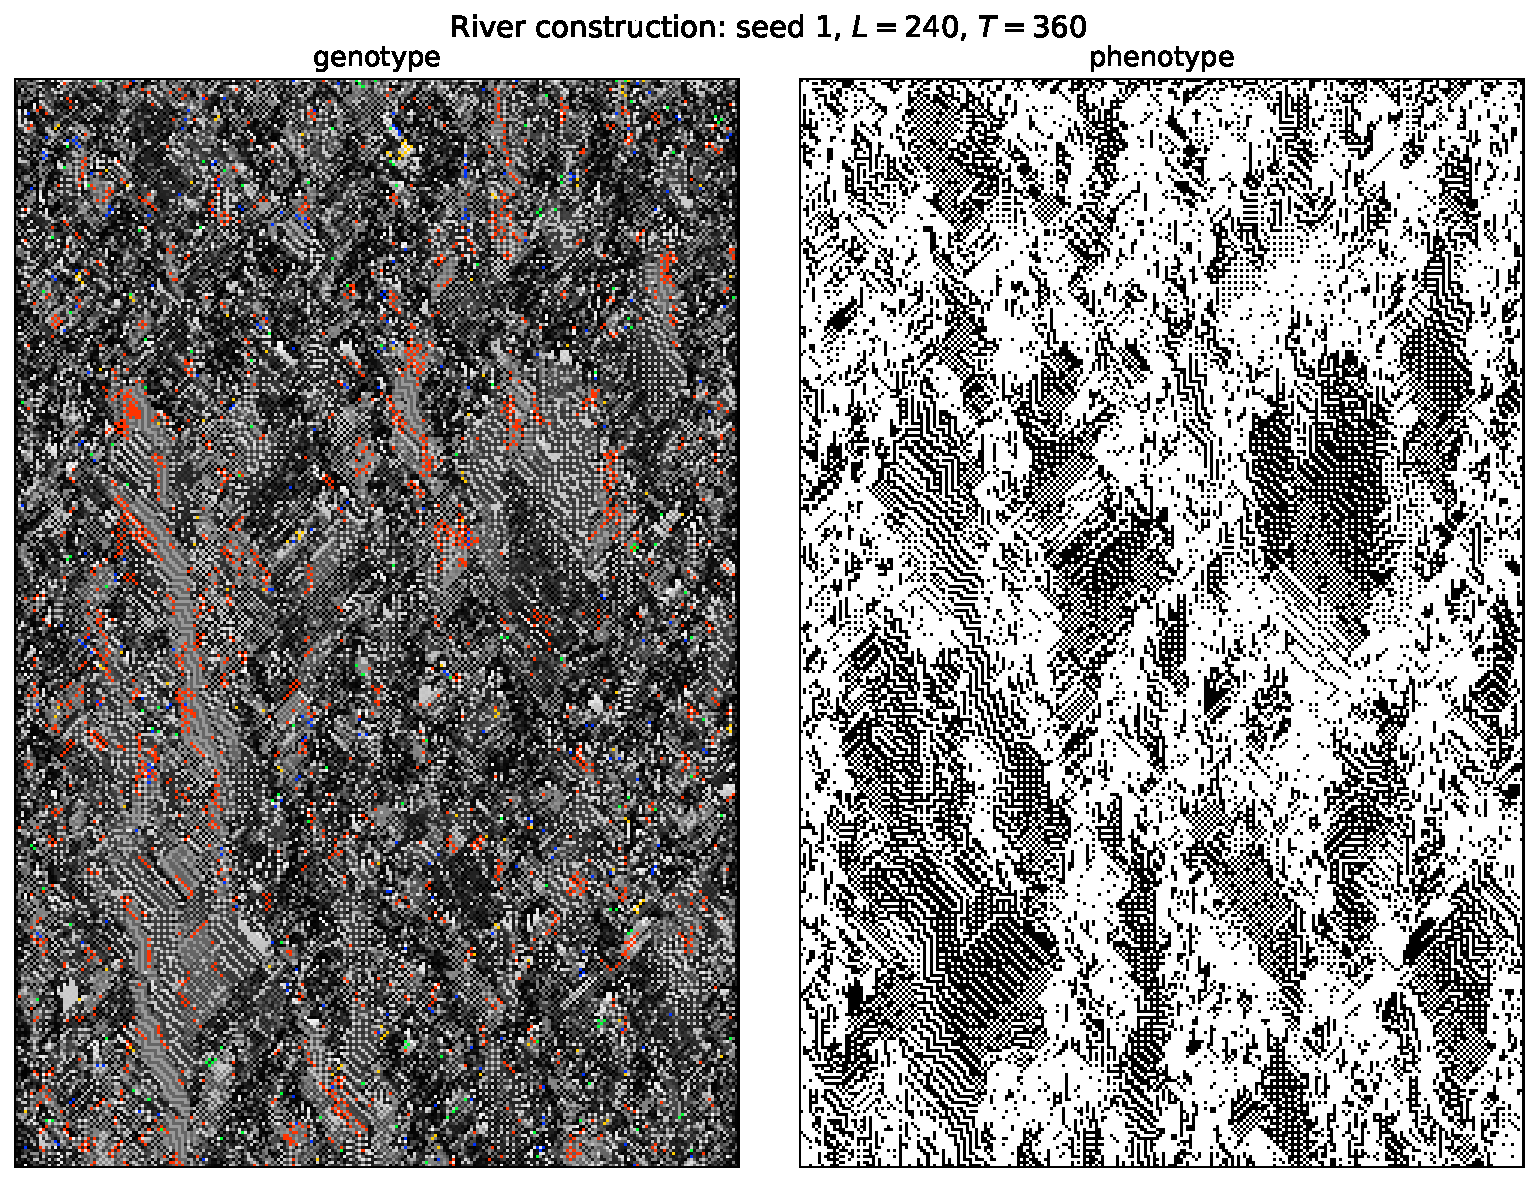
\includegraphics[width=\linewidth]{figures/river.pdf}
\caption{A \emph{river}: a composed operator sustains a reproducible
structure. The offset-$+2$ propagator, composed with a phenotype-reading,
four-candidate, first-match template construction (fallback: the all-zero
rule), produces in
each of six seeds a coherent band of alternating phenotype (bottom row)
drifting through a disordered background (genotype top, six seeds; genotype
coloured by rule as in Figures~\ref{fig:regimes}--\ref{fig:eoc}---greyscale by
byte value, with well-known ECAs highlighted, red~$=$~Rule~110). The band's
trajectory varies with the seed; its presence does not.
Where the bare rotations collapse or cycle (Figure~\ref{fig:eoc}), this
composition holds an off-critical structure for the length of the run.}
\label{fig:river}
\end{figure}

\section{Limits of the Tested Distance and Complexity Measures}
\label{sec:metrics}

\begin{empiricalfinding}[label={obs:metrics}]{The tested per-trajectory metrics do not separate the parity classes}
The classification is a conjugacy invariant of $\sig$---its cycle type---while
the complexity and compression measures we tried read a single rule's bits or one
space--time trajectory without explicitly encoding $\sig$. In our tests these
measures did not recover the parity classification: a population count reads a collapsed-but-maximally-selected
field as nearly dead; a frozen periodic genotype scores a lower statistical
complexity $C_\mu$ \parencite{crutchfield1989inferring} than Rule~110; gzip rates
a self-similar rule as noise. This is a negative result about the tested
summaries, not an impossibility theorem for trajectory-based inference.
\end{empiricalfinding}

\section{Discussion}
\label{sec:discussion}

The survey (Figure~\ref{fig:eoc}) exposes a sharp behavioural split within a
family of provably fixed-point-bearing operators: only the single 8-cycles
(offset $\pm 1$, $\pm 3$) sustain a high-diversity phase, while offset $\pm 2$ and
$\pm 4$ collapse. A reader is entitled to ask whether that phase sits at a
\emph{critical point}---tuned between an ordered and a disordered phase, as CA
complexity is often supposed to \parencite{langton1990computation}. We test this
with a finite-size scan and then ask whether the sustained diversity is spatially
organised into coexisting dynamical regimes.

\begin{empiricalfinding}[label={find:crossover}]{No finite-size evidence of a critical point over the tested range}
The natural control parameter is the \emph{propagator fraction} $q$ ($q = 0$ all
blend, $q = 1$ all propagator, offset $+2$). Across widths $L = 30$--$240$ (32
seeds each) the genotype activity $a_G(q)$ rises \emph{smoothly}, well described
by a logistic crossover ($R^2 > 0.99$, Figure~\ref{fig:phase}a); its width does
not shrink over the tested sizes ($w \approx 0.13$, $w \sim L^{-0.04}$). The
size-scaled run-to-run spread $L\,\mathrm{Var}(a_G)$
(Figure~\ref{fig:phase}b), used as a finite-size susceptibility proxy,
\emph{peaks} inside the crossover band, but the peak drifts in location
($q=0.75,0.50,1.00,1.00$ as $L$ increases) and grows ${\sim}5.7\times$ from the
smallest width to the largest; for the two largest sizes its maximum lies at
the sampled boundary $q=1$, so no convergent interior peak is resolved. Together
with the non-shrinking logistic width and absence of a Binder-cumulant crossing,
the scan provides no finite-size evidence for a sharpening transition over
$L=30$--$240$. These results support a broad crossover, plausibly
influenced by seed-dependent residence times, rather than a confirmed critical
point; they do not exclude different scaling outside the tested range.
\end{empiricalfinding}

\begin{empiricalfinding}[label={find:littoral}]{A finite-width intermediate-activity band}
An intermediate-activity band ($0.15 \le a_G \le 0.60$) has a \emph{lower} edge
robustly at $q \approx 0.1$---stable under both system size and threshold---while
its upper edge is threshold-dependent, because $a_G$ saturates gradually rather
than jumping (the band spans $q \approx 0.1$ to $0.4$--$0.5$). This finite-width
crossover is what we call a \emph{littoral edge}: a descriptive name for a shore
of finite width, not a thermodynamic phase boundary.
\end{empiricalfinding}

\begin{definition}[Isolated-rule activity score]\label{def:activity}
The \emph{activity score} of a rule is the mean per-step cell-change fraction
over the final $150$ steps of a $300$-step ordinary ECA run on a periodic line
of width $300$. Every rule uses the same density-$1/2$ pseudorandom initial
condition (seed $1$). This finite-run measure is distinct from the static
truth-table balance $\lambda$ (\secref{sec:lambda}). Ordered rules score near
$0$; Rule~$110$ scores approximately $0.42$, and several standard chaotic rules
score approximately $0.50$. The score orders activity levels but does not by
itself distinguish complex from chaotic dynamics.
\end{definition}

Tinting the genotype by this score (Figure~\ref{fig:tint}) resolves the
intermediate field into coexisting low- and high-activity domains whose
boundaries trace filamentary sets through $1{+}1$-dimensional spacetime---objects
\emph{analogous to} the domain boundaries of computational mechanics
\parencite{crutchfield1989inferring,shalizi2001computational}, here obtained by
thresholding a scalar tint rather than by predictive equivalence.

\begin{empiricalfinding}[label={find:walls}]{Filamentary walls have elevated genotype churn}
The activity field resolves into ordered and chaotic domains separated by
\emph{fractal-like walls} (Figure~\ref{fig:interface}; box-counting dimension
$D \approx 1.5$--$1.7$ over $L = 128$--$768$, a handful of seeds). Those walls are
the locus of elevated \emph{genotypic} change: measuring the row-to-row rewrite
rate by region (Table~\ref{tab:churn}), the wall churn exceeds the chaotic
interior in all $32$ committed operator/width/seed fields and exceeds
\emph{both} interiors in $24$. At $L = 256$, offset $+1$ gives $0.80$ at the
wall against $0.81$ (ordered) and $0.73$ (chaotic); the corresponding wall is
the maximum region for $\sigma=16250374$ and the river. The chaotic domain has
the lowest aggregate churn for every operator and width (and in $29$ of the
$32$ individual fields), so the wall---where ordered abuts chaotic---is
consistently more rewritten than the chaotic interior, though not universally
more than the ordered one. The walls are not compositionally special (no rule
class enriched; Rule~110 is, if anything, depleted), so the distinction is
dynamical rather than a difference in rule composition. The interface analysis
is exploratory: it uses a handful of seeds and a fixed-boundary variant, and
the denser river boundary ($D\approx1.8$ versus $1.5$--$1.7$) is an unmatched
comparison that does not establish an effect of genotype--phenotype coupling.
Whether rewriting transports or combines information \emph{along} the walls is
not tested here.
\end{empiricalfinding}

\begin{figure}[tb]
\centering
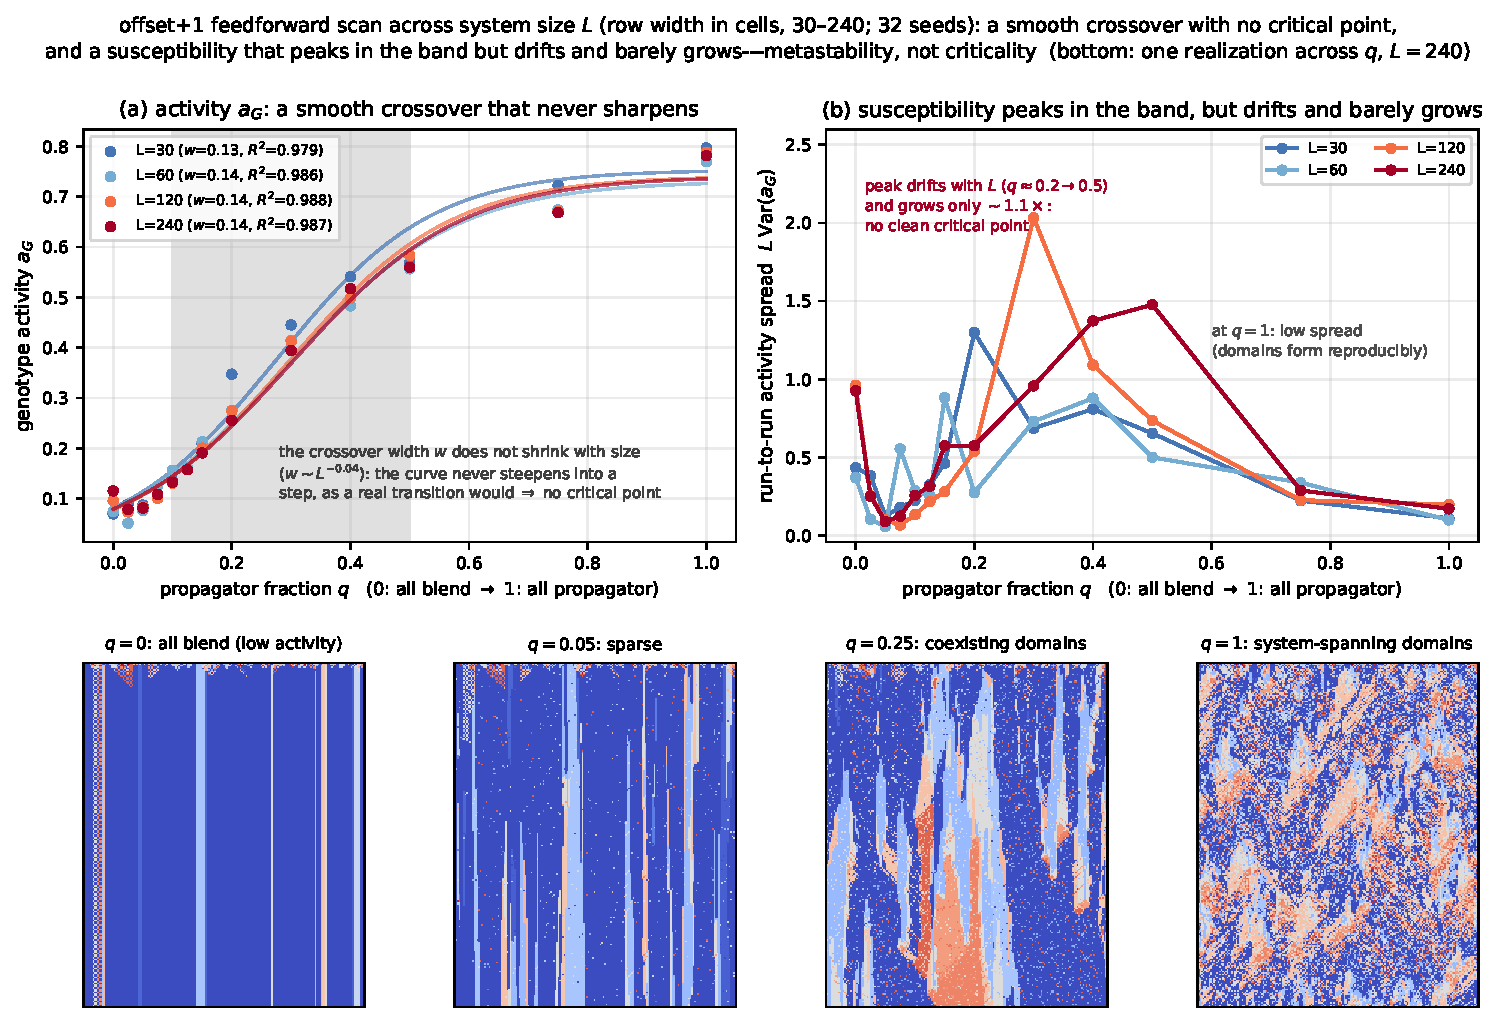
\includegraphics[width=\linewidth]{figures/eoc_phase.pdf}
\caption{\textbf{No finite-size evidence of a critical point over the tested
range.} Offset $+1$ feedforward finite-size scan against the
propagator fraction $q$ ($0$: all blend, $1$: all propagator). $L$ is the
\emph{system size}---the lattice width in cells; the scan spans $L = 30$--$240$
(32 seeds each), because a genuine transition sharpens as $L$ grows while a
crossover does not. \textbf{(a)}~genotype activity $a_G$ with logistic fits
($R^2 > 0.99$); the crossover width does not shrink over these sizes
($w \sim L^{-0.04}$). \textbf{(b)}~the size-scaled run-to-run spread
$L\,\mathrm{Var}(a_G)$ is used as a susceptibility proxy: it peaks inside the
band, but its maximum moves from $q=0.75$ to $0.50$ and then to the sampled
boundary $q=1$ for the two largest sizes; its height grows ${\sim}5.7\times$.
\textbf{(c)}~finite-horizon collapse becomes rarer with size.
\textbf{(d)}~the Binder cumulant has no common crossing. Together these
diagnostics support a broad crossover rather than a confirmed critical point.
Bottom: one paired realisation ($L = 240$, single seed) tinted by isolated-rule
activity at $q=0$, $0.05$, $0.25$, and $0.75$.}
\label{fig:phase}
\end{figure}

\begin{figure}[tb]
\centering
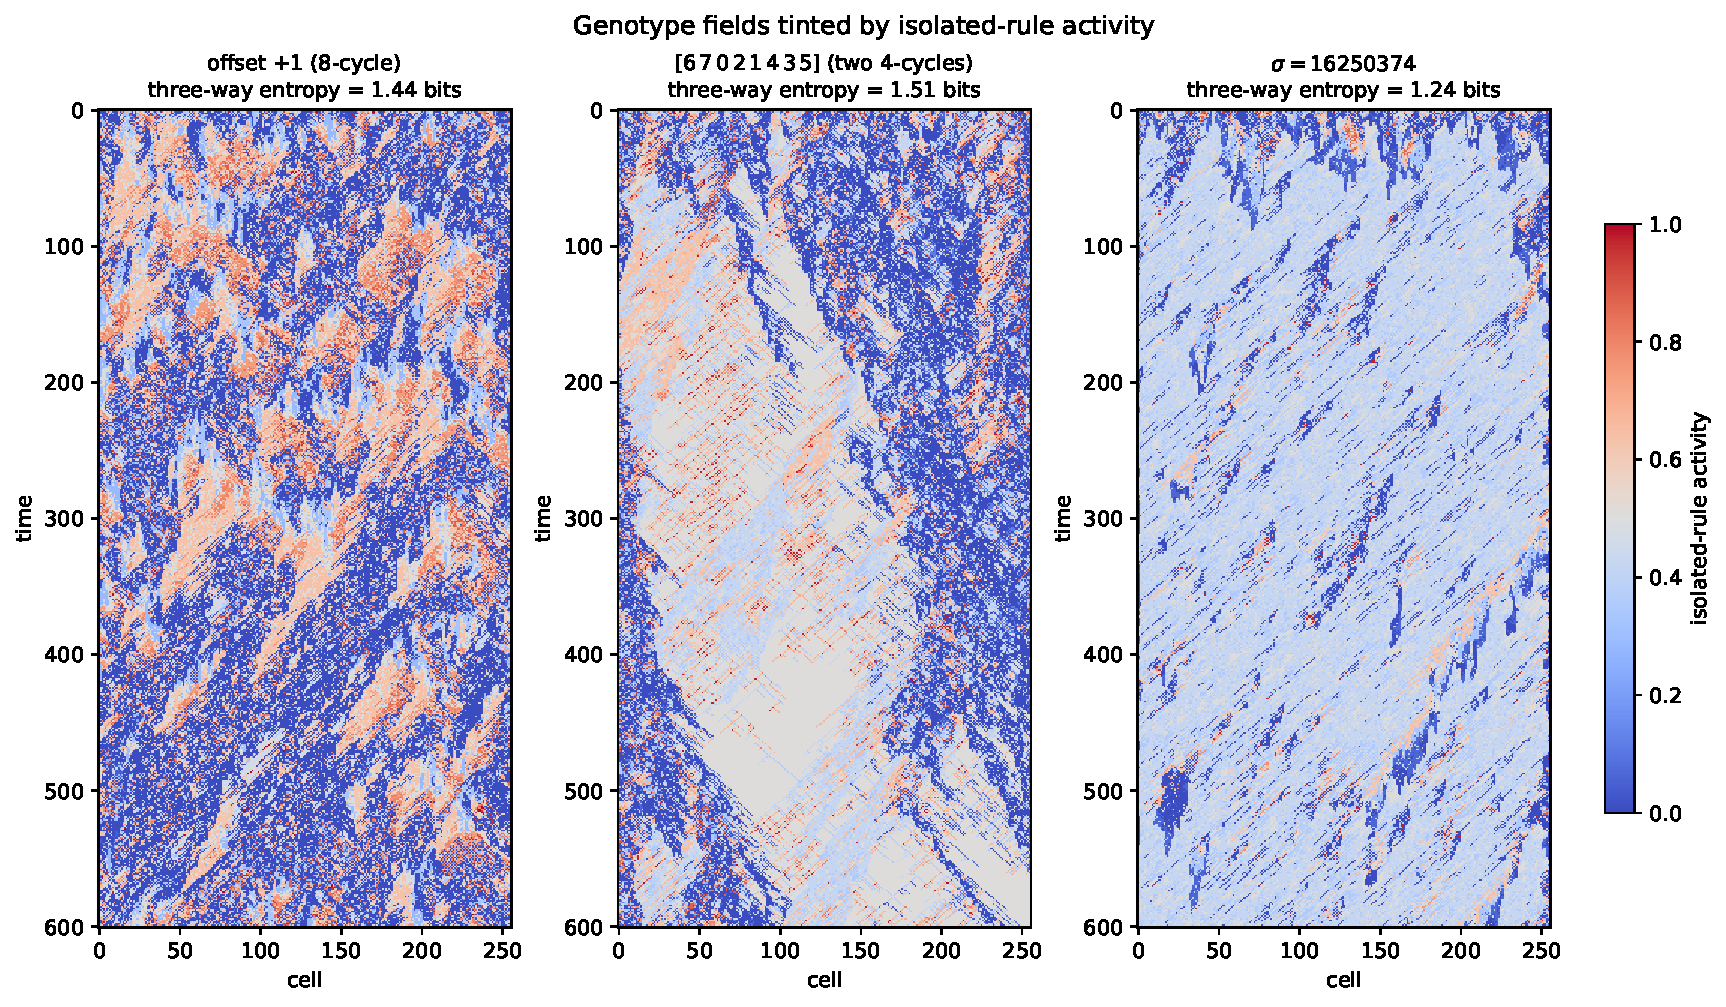
\includegraphics[width=\linewidth]{figures/eoc_tint.pdf}
\caption{\textbf{The genotype as a map of activity regimes.} Genotype spacetime
fields (fixed-boundary variant) tinted by each rule's \emph{isolated-rule
activity score} (Definition~\ref{def:activity}; blue $=$ low near $0$, pale $=$
intermediate near $0.4$, red $=$ high near $0.5$ and above). Which active regime
pairs with the low-activity background depends on the operator, and the three-way
balance differs sharply (entropy in bits, in title): offset $+1$ (the 8-cycle
survivor) mixes low with high-activity chaotic rules in a \emph{fine} texture;
the two-4-cycle $[6\,7\,0\,2\,1\,4\,3\,5]$---the standard-order form of the
historical offset$+2$ exemplar---forms \emph{large coherent}
intermediate-activity domains
with sharp walls, the most balanced regime mix (entropy $1.51$); and
$\sigma = 16250374$ is dominated by the intermediate complex Rule~110. The score
orders the regimes but does not by itself separate complex from chaotic.}
\label{fig:tint}
\end{figure}

\begin{figure}[tb]
\centering
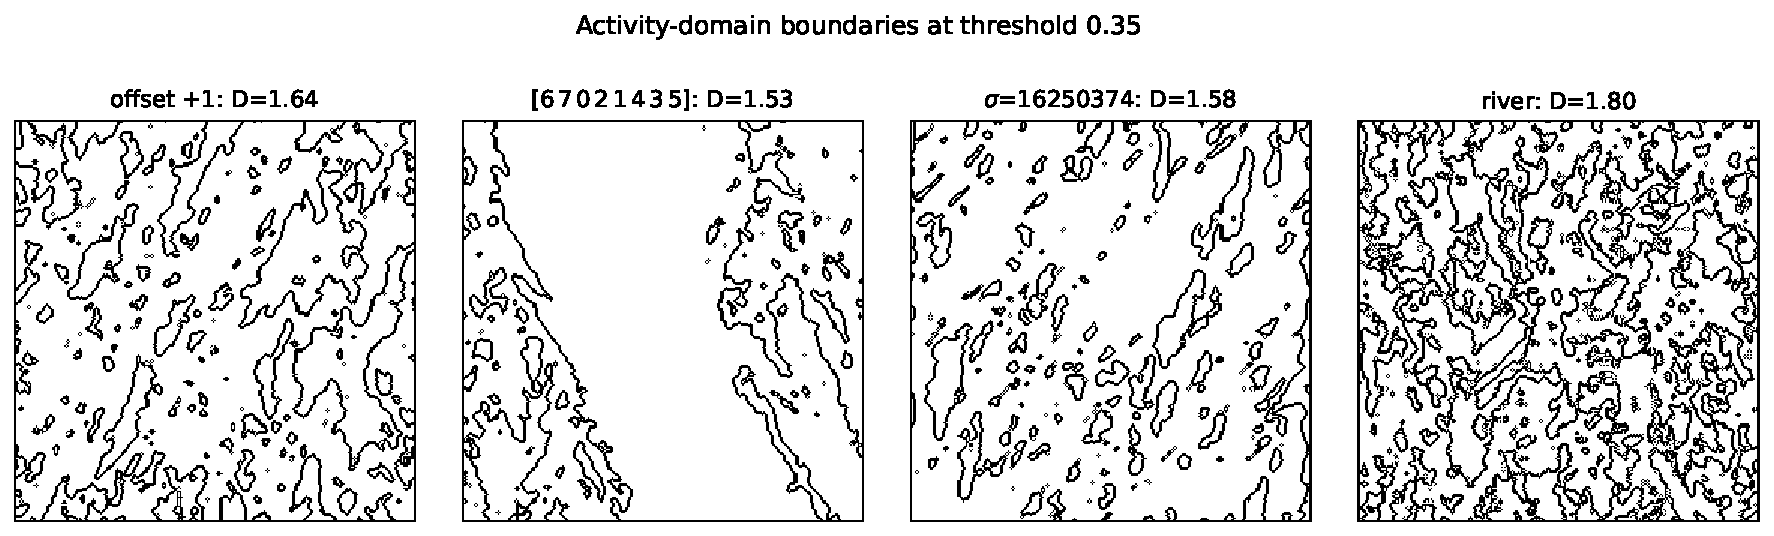
\includegraphics[width=\linewidth]{figures/eoc_interface.pdf}
\caption{\textbf{Activity-domain walls.} The boundary (black) between low- and
high-activity regions, traced through the $1{+}1$-dimensional spacetime diagram at
$L = 256$. Offset $+1$, the two-4-cycle
$[6\,7\,0\,2\,1\,4\,3\,5]$, and $\sigma = 16250374$ carry fractal-like
boundaries ($D \approx 1.5$--$1.6$); the phenotype-coupled river carries a
denser one ($D \approx 1.80$, an unmatched comparison as it couples phenotype).
The dimension is stable across $L = 128$--$768$ (offset $+1\approx1.67$, the
two-4-cycle $\approx1.50$, $\sigma\approx1.54$, and river $\approx1.79$; box
sizes $2$--$64$). Collapsed operators (e.g.\ offset $+4$) carry none. These
walls are also consistently more rewritten than the chaotic-domain interior
(Discussion). Exploratory: a handful of seeds, fixed-boundary variant.}
\label{fig:interface}
\end{figure}

\begin{table}[tb]
\centering
\caption{\textbf{Genotype churn by region}---row-to-row rewrite rate of the rule
field (fraction of cells whose ECA rule changes from the row above), at
$L = 256$, mean over the committed seeds. The wall exceeds the chaotic
interior for every operator; for offset $+1$, the ordered interior is slightly
higher. Wall extraction is the threshold-and-smooth procedure of
Figure~\ref{fig:interface}; reproducible from the committed fields
(\texttt{plot\_eoc\_churn.py}).}
\label{tab:churn}
\begin{tabular}{lccc}
\toprule
Operator & Wall & Ordered interior & Chaotic interior \\
\midrule
offset $+1$          & $0.80$ & $0.81$ & $0.73$ \\
$\sigma = 16250374$  & $0.71$ & $0.68$ & $0.57$ \\
river                & $0.99$ & $0.97$ & $0.96$ \\
\bottomrule
\end{tabular}
\end{table}

\section{A Sampled Edge of Chaos}
\label{sec:eoc-compute}

If the filaments are domain boundaries they are candidate \emph{wires}. The
natural question is not which rules compose them---in our data the complex rules
are not enriched there---but whether information is \emph{transported along} them
and \emph{combined where they collide} \parencite{mitchell1993revisiting}. Rather
than defer this entirely, we take a few samples.

We read both notions off the binary activity field as local transfer entropy
\parencite{lizier2008local}: the apparent transfer entropy from a spatial
neighbour into a cell, conditioned on the cell's own past, scores directed
\emph{transport}; the \emph{synergy} of the two neighbours---their joint
predictive contribution beyond the sum of their separate ones---scores
\emph{combining} (Figure~\ref{fig:eoc-schema}). On the offset$+1$ field the directed transfer entropy
concentrates on the filaments (about five-fold over the domain interiors) and
collapses to near zero under a source time-shuffle that preserves marginals, so
the transport is genuine and not a by-product of where the field happens to
change; Rule~$110$, as a positive control, shows the same signature.

\begin{figure}[tb]
\centering
\begin{tikzpicture}
\node[inner sep=0.4pt, draw=black!25] (p) {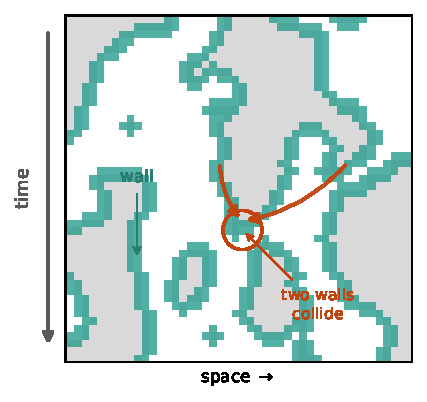
\includegraphics[width=56mm]{figures/eoc_patch.pdf}};
\node[font=\footnotesize, anchor=south] at (p.north)
  {\textbf{(a)} a real patch (offset$+1$): activity domains and their walls};
\end{tikzpicture}
\\[3mm]
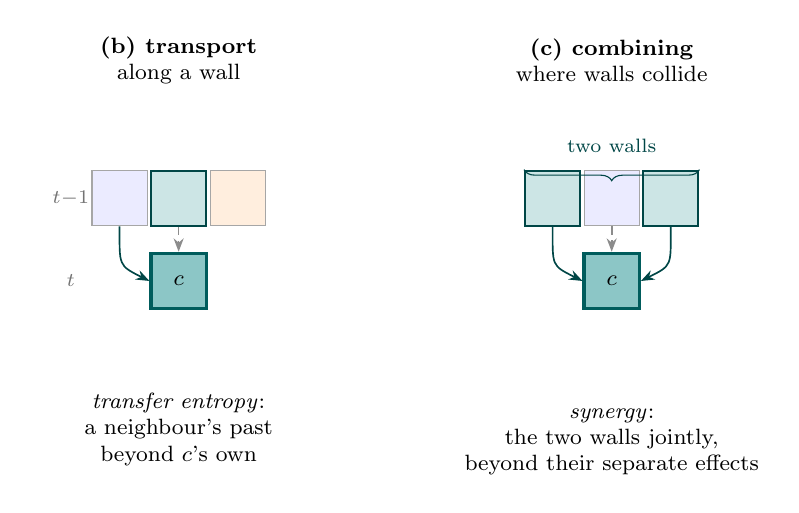
\begin{tikzpicture}[font=\footnotesize, >={Stealth[length=1.6mm]},
  cell/.style={draw=black!35, minimum size=7mm, inner sep=0},
  ord/.style={cell, fill=blue!8},
  cha/.style={cell, fill=orange!13},
  wall/.style={cell, fill=teal!20, draw=teal!55!black, thick},
  tgt/.style={cell, fill=teal!45, draw=teal!72!black, very thick},
  te/.style={-{Stealth[length=1.7mm]}, teal!55!black, semithick},
  own/.style={-{Stealth[length=1.7mm]}, black!45, semithick, densely dashed},
  rowlab/.style={font=\scriptsize\itshape, black!55},
  blurb/.style={align=center, font=\footnotesize}]
% Panel (a): transport
\node[blurb] at (0.75,1.75) {\textbf{(b) transport} \\ along a wall};
\node[ord]  (aP0) at (0,0)        {};
\node[wall] (aP1) at (0.75,0)     {};
\node[cha]  (aP2) at (1.5,0)      {};
\node[tgt]  (aC)  at (0.75,-1.05) {$c$};
\node[rowlab] at (-0.62,0)     {$t{-}1$};
\node[rowlab] at (-0.62,-1.05) {$t$};
\draw[own] (aP1) -- (aC);
\draw[te]  (aP0.south) .. controls +(0,-0.5) and +(-0.4,0.2) .. (aC.west);
\node[blurb, text width=36mm, anchor=north] at (0.75,-2.35)
  {\emph{transfer entropy}:\\ a neighbour's past beyond $c$'s own};
% Panel (b): combining
\begin{scope}[xshift=55mm]
\node[blurb] at (0.75,1.75) {\textbf{(c) combining} \\ where walls collide};
\node[wall] (bP0) at (0,0)        {};
\node[ord]  (bP1) at (0.75,0)     {};
\node[wall] (bP2) at (1.5,0)      {};
\node[tgt]  (bC)  at (0.75,-1.05) {$c$};
\draw[decorate, decoration={brace, amplitude=4pt, mirror}, teal!55!black]
  (bP0.north west) -- node[above=2.5pt, font=\scriptsize, teal!55!black] {two walls} (bP2.north east);
\draw[own] (bP1) -- (bC);
\draw[te]  (bP0.south) .. controls +(0,-0.5) and +(-0.4,0.2) .. (bC.west);
\draw[te]  (bP2.south) .. controls +(0,-0.5) and +(0.4,0.2)  .. (bC.east);
\node[blurb, text width=38mm, anchor=north] at (0.75,-2.55)
  {\emph{synergy}:\\ the two walls jointly, beyond their separate effects};
\end{scope}
\end{tikzpicture}
\caption{\textbf{How the two measures read a filament.} \textbf{(a)}~A real
space--time patch from the synthetic family (offset$+1$): low- and high-activity
domains (white/grey) meet along thin walls (teal), with one wall and one collision
marked. In the schematics each cell $c$ is predicted from its own past (dashed)
and its two spatial neighbours' pasts (teal); tints mark the low- (blue) and
high-activity (orange) domains a wall separates. \textbf{(b)}~\emph{Transport} is
the directed transfer entropy from a neighbour into $c$ beyond $c$'s own past,
elevated on the walls. \textbf{(c)}~\emph{Combining} is the \emph{synergy} of the
two neighbours---their joint contribution beyond the sum of their separate
ones---probed where two walls collide. History length one; conditioning on the
own past removes what the wall merely carries forward in time.}
\label{fig:eoc-schema}
\end{figure}

To ask whether combining is a property of the \emph{edge} rather than of the
operator alone, we sample a synthetic order--chaos family. The neighbour-blend
interrupter (\secref{sec:interrupter}, fraction $q$) tunes toward order; an
independent, seeded stochastic rule-flip applied to the genotype each step
(rate $p$) tunes toward chaos; the bare propagator sits between them at
$q=1,\,p=0$. Figure~\ref{fig:eoc-compute} reports filament combining across this
family.

\begin{observation}[label={obs:eoc-compute}]{Combining peaks at a literal edge of chaos}
Averaged over eight seeds, filament synergy rises out of the ordered regime,
reaches a maximum at an intermediate blend fraction ($q\approx0.4$), and decays
monotonically through the bare propagator into the noise-driven regime.
Combining is thus largest at a transitional regime---a literal edge of chaos in
the sense of \textcite{langton1990computation}---and is suppressed by both
over-ordering and disorder. The bare offset$+1$ operator sits near this maximum,
on its mildly descending side. This is a first sample and not a map: it rests on
one synthetic family, one information measure (the co-located transport score is
confounded on the chaotic flank, where noise manufactures transitions), eight
seeds, and a rise at the ordered extreme that is partly a sparsity effect.
\end{observation}

Whether computation genuinely flows down the littoral filaments of these
diagrams---beyond these few samples---remains a question for another paper.

\begin{figure}[tb]
\centering
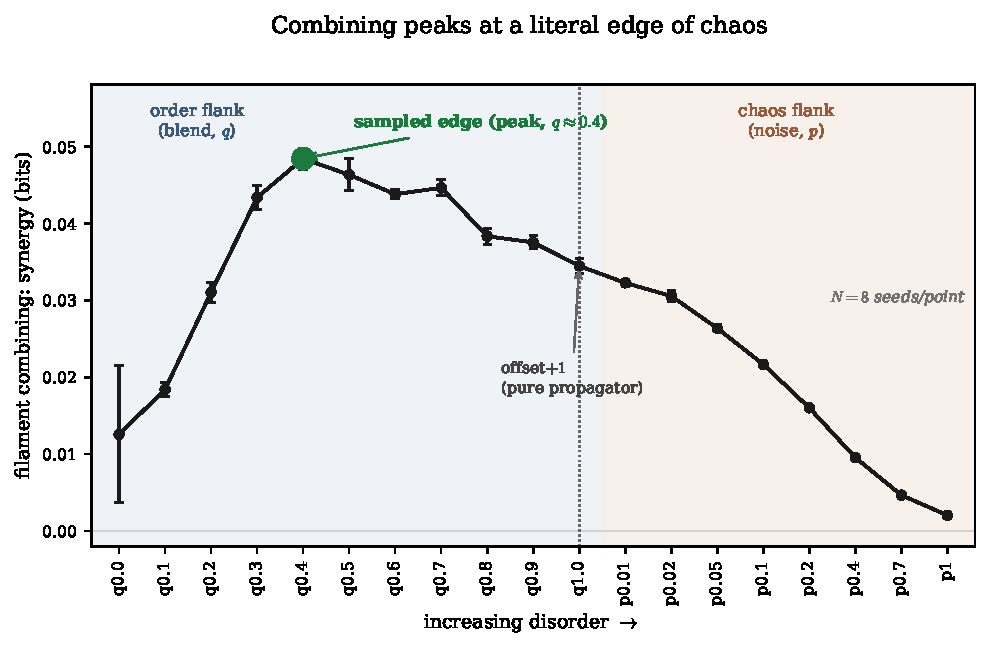
\includegraphics[width=0.85\linewidth]{figures/edge_of_chaos_curve.pdf}
\caption{\textbf{A sampled edge of chaos.} Filament \emph{combining} (synergy of
the two spatial neighbours' contributions to a cell's genotype rewrite, in bits)
across a synthetic order--chaos family: the blend interrupter tunes toward order
(fraction $q$), a seeded stochastic rule-flip tunes toward chaos (rate $p$), with
the bare offset$+1$ propagator between them. Points are means over $N=8$ seeds;
bars are $\pm$SEM. Combining peaks at an intermediate regime ($q\approx0.4$) and
decays into both order and chaos; the bare operator sits near, but below, the
peak. Within this family the peak exceeds both the ordered ($p<0.01$) and chaotic
($p<10^{-8}$) extremes and the bare operator itself ($q=1$; $p<10^{-5}$, Welch
$t$-tests), and the chaotic flank decays monotonically (Spearman $\rho=-0.98$,
$n=72$). These significances are within a single family and a single measure;
generality across operators is untested.}
\label{fig:eoc-compute}
\end{figure}

\section{Limits}
\label{sec:limits}

The theorems are the Boolean case and are exact; the dynamical claims are
narrower and empirical. The census and the sustained-diversity behaviour are
reported for a single spatial coupling ($S_8$, radius one, one value map) at
limited seed counts, and invite a fuller treatment. \secref{sec:discussion}
takes up the local, structural reading and reports an exploratory
interface-dimension statistic under its own stated caveats (few seeds,
fixed-boundary variant); beyond it we report no perturbation-spreading or
entropy-rate statistics.
The empirical components use different fixed sample sizes: three seeds per
operator in the census, two per rotation in the survey, six for the river and
Rule~110 comparison, and $32$ per parameter cell in the finite-size scan; the
interface analysis uses the smaller samples stated with that result.
Illustrative diagrams use pinned representative seeds. All are reproducible
from the accompanying package. The
substrate the object sits in is not itself new (\secref{sec:object}); $\lambda$
is one heuristic among several \parencite{wuensche1999classifying}, and we
make no claim that balance implies any particular dynamics---only that here
balance is \emph{derived}. What is new, and what we rest the paper on, is the
object of Equation~\eqref{eq:prop} and the fixed-point structure that forces
every fixed rule to be balanced, $\lambda = 1/2$, as a matter of proof.

\section{Conclusion}
\label{sec:conclusion}

The characterisation promised at the outset (\secref{sec:object}) has two
halves. The
first is static and exact: which operators possess fixed points (the
all-even ones), how many ($2^k$), and where they lie (balanced,
$\lambda = 1/2$, always). The second is empirical and tentative. Because
every fixed point sits at $\lambda = 1/2$, that parameter is silent on the
difference between an operator whose field stays diverse and one whose field
collapses; the distinct-rule count is not, and in our
runs it separates the two across the rotation family by more than an order of
magnitude (Figure~\ref{fig:lambda}). The same observable offers a suggestive
reading of the search that produced the family, reported both as a
representative run and as a fixed six-seed sample (\secref{sec:limits}). The
operator of Figure~\ref{fig:regimes} that comes to be dominated by
Rule~110---a conventional target in a search for computationally distinguished
behaviour---concentrates the field onto it and pays for it in diversity.
At the representative seed, $39\%$ of its genotype cells are Rule~110 and it
sustains $16$ distinct rules, against a foil that holds Rule~110 below $1\%$
and sustains $33$; over the six-seed sample the ordering is unchanged---Rule
110 $35\%$ (range $31$--$39\%$) versus $0.2\%$ ($0$--$0.2\%$), sustained diversity
$15$ versus $23$. On this pair, recovering a universal rule and sustaining a
diverse population pull against each other---a suggestion worth testing at
scale, not a law we have established.

\paragraph{Data and code availability.} The generated numerical data underlying
the tables, figures, and reported summary statistics, together with the code and
documented commands needed to regenerate them, are publicly available at
\texttt{https://github.com/tothedarktowercame/mmca-clj} (commit
\texttt{9f68611ca6d512006a610e9712b7ccc3bf1dfd7b})---a standalone,
dependency-light Clojure port of the MetaCA dynamics whose \texttt{README} gives
the complete reproduction command and commands for individual figure groups.
The classification and balance theorems are
formally verified in Lean~4 with Mathlib at
\texttt{https://github.com/tothedarktowercame/mathlib4}, branch \texttt{darktower}
(commit \texttt{bc34d8cec27216aae1d3cd511a9950ab1bce3575}), in
\texttt{DarkTower/Patterns/Propagator.lean}: the cycle-parity criterion as
\texttt{hasAlternatingColouring\_iff\_cycleType\_even} and the $\lambda = 1/2$
balance as \texttt{alternatingColouring\_true\_card\_eq\_four}. The same file
also contains executable regressions for both hand calculations, including the
displayed-position versus numerical-neighbourhood indexing contrast.

\paragraph{Generative-AI disclosure.} Anthropic Claude Opus~4.8 and OpenAI
Codex coding agents \parencite{anthropic_claude,openai_codex} assisted in an
iterative, human-supervised workflow with manuscript editing, software
implementation, test construction, and adversarial checks. The author reviewed
the resulting prose and code, reran the reported computations and formal
checks, and accepts full responsibility for the manuscript. Product information
was accessed on July~25, 2026.

\printbibliography
\end{document}
